% Chapter

\chapter{Traversal of Yellow Fever Vaccine Strain 17D Seed Lineages by Deep Sequencing Reveals Limited and Stable Patterns of Subpopulation Diversity}

\section{Abstract}
Attenuated phenotypic properties of the 17D vaccine lineage are well described and standardized using a seed-lot system developed in 1945; however, the discrete mechanisms giving rise to these features are poorly understood. Quasispecies theory is a useful paradigm by which to understand the influence of viral diversity upon vaccine attenuation by considering evidence that low diversity is a characteristic of attenuated viruses. To investigate these patterns for the \gls{yfv} vaccine, an archived panel of 17D derivative seed and vaccine lots from different producers was assembled, representing the 17D substrains 17D-204, 17D-213, and 17DD. Massively parallel sequencing analysis was performed to assess the stability and homogeneity of subpopulation identity along divergent branches across the entire 17D lineage. Within each substrain, concordance of diversity and variant structure was observed; these patterns were recapitulated between substrains, but to a lesser degree. The results indicate that, despite production of multiple substrains of live-attenuated 17D vaccine, there is considerable homogeneity of the vaccine across multiple subculture passage histories, and that the seed-lot system is very effective at controlling the apparent diversity of the vaccine. Overall, the results suggest that \gls{ngs} provides a technique to evaluate and resolve patterns of population structure in live attenuated vaccine preparations.

\section{Introduction}
All \gls{yfv} vaccines in current use are derived from the 17D lineage, developed by the Rockefeller Foundation in 1937 \parencite{Theiler:1937wy,Theiler:1951ti}. Following derivation of the 17D vaccine strain from the parental Asibi, the virus underwent a varied passage history with three substrains recognized, named 17D-204, 17DD and 17D-213 based on the passage level that they were derived \parencite{WorldHealthOrganization:2010wo}. Briefly, the 17DD substrain was derived from 17D at passage 195, and is currently manufactured only in Brazil. The 17D-204 substrain refers to all vaccines derived from the original 17D strain at passage 204. The 17D-213 substrain refers to a derivative of 17D-204 developed by the \gls{rki} to be free of contamination by avian leucosis virus; 17D-213/77 is the prototype of this substrain, and is the primary reference seed of the \gls{who} \parencite{Bres:1987wl}. Over the last 75 years 17D vaccine has been produced in 14 different countries (Australia, Brazil, China, Colombia, France, Germany, India, Netherlands, Nigeria, Russia, Senegal, South Africa, United Kingdom, and United States) \parencite{Monath:2013cu}. Since the lineage relationships of all \gls{yfv} vaccines by passage level is exactly known, the tree represented by the strains represents a dataset by which to interrogate the stability of the 17D genotype by traversal of known passage histories.

In early development of \gls{yfv} vaccines, phenotypic stability was investigated by \emph{in vivo} classical methods. 17D was shown to regain neurotropism to monkeys if serially passaged in mouse brain \parencite[129]{Theiler:1951ti}. \Gls{ih} passage of the French neurotropic vaccine strain, a competing live-attenuated product in Rhesus macaques revealed that viscerotropism could be efficiently selected and enhanced, leading to an early speculation as to the inherent diversity in tissue-fixed viral vaccines \parencite{FINDLAY:1935vu}. One early field trial in a Brazilian cohort observed a loss of immunogenicity for a 17D-derived vaccine batch produced from seeds at extended subculture levels \parencite{Soper:1938tb}. 

These safety concerns prompted the development of a seed-lot system for the vaccine in 1945, a regulatory structure that remains in use today. Production lots of each 17D vaccine are derived from first a primary, then secondary, seed material qualified to possess acceptable phenotypic and genotypic characteristics \parencite{WorldHealthOrganization:2010wo}. Because production lots of vaccine arise by single egg passage from secondary seed virus, subculture levels of production batches relative to the parental strain are exactly known, providing a reference by which to interrogate stability and consistency of the vaccine lineage over time with modern tools. A collection of vaccines and seeds from the 17D-204 and 17DD substrains were compared by T1 \gls{rna} oligonucleotide fingerprinting, revealing slight differences in electrophoretic patterns between the substrains \parencite{Monath:1983uk}. 

The French Stamaril® vaccine (17D-204 substrain) was analyzed by sequence, multiplication kinetics, and plaque size distribution, revealing considerable stability for a set of production lots manufactured between 1990 and 2002 \parencite{Barban:2007hi}. Limited divergence of consensus sequence is observed across the entire 17D lineage; Bayesian phylogenetic analysis of consensus sequences for a set of 17D vaccines resolved clustering patterns by substrain history \parencite{Stock:2012gp}.

Quasispecies theory is now a prominent framework for understanding the lifecycle of \gls{rna} viruses such as \gls{yfv}, which replicate under short generation times by means of error-prone \gls{rna}-dependent-\gls{rna}-polymerases \parencite{Domingo:2012hw}. Briefly, low-frequency sequence variants are observed to arise during the viral lifecycle, underlying a dominant genotype. The presence and relative abundance of these variants have been shown to be possible fitness determinants for the viral population, which is considered an aggregate unit of selection. This was shown most dramatically for \index{Viruses, Miscellaneous!\Acrfull{pov}}\gls{pov}, in which chemical mutagenesis restored neuropathogenicity of a strain bearing a high-fidelity polymerase and consequently impaired fitness \parencite{Vignuzzi:2006ju}. For \gls{yfv}, a strain of the 17D vaccine was estimated to accumulate between $1.9 \times 10^{-7}$ and $2.3 \times 10^{-7}$ mutations per replicated genome, assessed by Sanger methods \parencite{Pugachev:2003fj}. The potential significance of this feature to the safety profile of 17D has not been determined experimentally, however since viral subpopulations are hypothesized to facilitate adaptation to within-host infection barriers, low mutational rates or content for \gls{yfv} vaccines are desirable to avoid the potential for \gls{wt} reversion once administered. Empirically derived vaccine strains such as 17D therefore represent an ideal context by which to investigate the association of viral diversity with phenotype. The availability of standardized vaccine strains permits the reconstruction of typical population structures that may define an attenuated vaccine genotype.

Massively parallel sequencing (\gls{ngs}) studies are frequently used to interrogate viral diversity, resolving subpopulation dynamics in response to various external factors, including tissue compartmentalization, immune system pressures, and pharmaceutical treatments \parencite{Nishijima:2012ew}. For vaccines, studies of this type have detected the presence of adventitious virus in commercial lots, after accomplishing low-coverage assembly ($<$100 mean reads per nucleotide site considered in the alignment) of a number of live-attenuated \gls{rna} virus vaccine strains, including \index{Viruses, Miscellaneous!\Acrfull{mev}}\gls{mev}, \index{Viruses, Miscellaneous!\Acrfull{rbv}}\gls{rbv}, and a 17D-derived vaccine lot \parencite{Victoria:2010kf}. 

For \gls{yfv} specifically, a deep sequencing study at high coverage ($>$5000 mean reads per nucleotide site considered) compared to \gls{wt} parental strain Asibi with a commercial lot of the 17D-204 substrain vaccine manufactured in the U.S. (YF-Vax\textsuperscript{\textregistered}) and revealed that the vaccine is in fact largely homogenous, and devoid of hidden diversity relative to the \gls{wt} strain \parencite{Beck:2014cm}. To investigate whether or not the same homogeneity is found in 17D vaccines manufactured by other producers, we have performed a deep sequencing study of primary and/or secondary seed lots, and some vaccine production lots for all modern substrains in present use, 17D-204, 17DD, and 17D-213. The assembled panel of seeds and vaccines represents production of \gls{yfv} vaccine from diverse subculture histories, permitting comparisons of both intra- and inter-lineage vaccine seed strains [Table \ref{origin_seeds} and Figure \ref{seeds_tree_tikz}]. Findings represent the most complete record of \gls{yfv} seed and vaccine relationships to date using these methods, and offers a framework by which the stability and consistency of the vaccine may be assessed over extended production histories \emph{in silico}.

\section{Results}
Origins and nomenclature for the strains considered are listed in Table \ref{origin_seeds}.
\subsection{17D-204 Substrain Coverages}
For the secondary seed 17D-204/United Kingdom/YFS/11, median coverage was 7491 (mean = 7275.4, \gls{sd}=1118.6). For the secondary seed 17D-204/South Africa/5114.15, median coverage was 7499 (mean = 7278.4, \gls{sd}=1198.4). For the Connaught vaccine strain 17D-204/USA/1995 (YF--Vax\textsuperscript{\textregistered} lot 4L51152), median coverage was 7400 (mean = 7286.2, \gls{sd}=1400.7). For the Sanofi-Pasteur vaccine strain 17D-204/USA/2012 (YF--Vax\textsuperscript{\textregistered} lot UH356AA), median coverage was 7534 (mean =7279.2, \gls{sd}=1154.9). For the Connaught vaccine strain 17D-204/USA/1995 (YF-Vax\textsuperscript{\textregistered} lot 4L51152), median coverage was 7400 (mean = 7286.2, \gls{sd}=1400.7). For the \gls{ndc} secondary seed 17D-204/USA/\gls{ndc}-6676, median coverage was 8704.5 (mean = 7279.2, \gls{sd}=4146.0). For the \gls{ndc} vaccine strain 17D-204/USA/\gls{ndc}-6677, median coverage was 7350 (mean = 7277.3, \gls{sd}=3582.6). 
	\subsection{17D-213 Substrain Coverages}
Consensus for the \gls{who} primary seed lot 17D-213/WHO/213-77, median coverage was 7160 (mean = 7280.7, \gls{sd}=1923.7). For the vaccine strain 17D-213/WHO/213-B2-81, median coverage was 7311 (mean = 7280.0, \gls{sd}=1595.2). For the vaccine strain 17D-213/Russia/SW13, median coverage was 7699 (mean = 7279.7, \gls{sd}=2400.9). For the vaccine strain 17D-213/Nigeria, median coverage was 7017 (mean=7278.3, \gls{sd}=3966.0). 
	\subsection{17DD Substrain Coverages}
For the secondary seed 17DD/Senegal/SLII-75-1, median coverage was 7574 (mean=7281.0, \gls{sd}=1230.7). For the vaccine strain 17DD/Colombia, median coverage was 7278 (mean = 7277.9, \gls{sd}=1216.3). 
	\subsection{Asibi Strain Coverage}
For the \gls{wt} parental strain Asibi, median coverage was 7311 (mean=7280.0, \gls{sd}=1595.2).
	\subsection{Consensus Sequences}
Consensus sequences for each vaccine virus were aligned to the \gls{wt} parental strain Asibi (Genbank accession AY640589), and compared to the \emph{de novo} Asibi sequence generated in parallel. For the entire set of 17D vaccine and seed strains considered, relative to the \gls{wt} Asibi strain, a set of 24 coding substitutions was recovered in common between all datasets (M-L36F, E-G52R, E-A170V, E-T173I, E-K200T, E-M299I, E-S305F, E-K331R, E-T380R, E-A407V, \gls{ns}1-L79F, \gls{ns}1-I307V, \gls{ns}2A-M118V, \gls{ns}2A-T167A, \gls{ns}2A-T172A, \gls{ns}2A-S183F, \gls{ns}2B-I37L, \gls{ns}2B-I109L, \gls{ns}3-D485N, \gls{ns}4A-V146A, \gls{ns}4B-I95M, \gls{ns}4B-Y231H, \gls{ns}5-E836K, \gls{ns}5-P901L) and two nucleotide substitutions in the 3’\gls{utr} (U10418C, A10847C) [Table \ref{main_subs_seeds}]. The current \gls{who} standard for \gls{yfv} vaccines lists 20 coding substitutions and four nucleotide changes in the 3’\gls{utr} (3’\gls{utr}) in reference to the parental strain Asibi that are conserved between all substrains of 17D [Table \ref{WHO_standard_YFV}] \parencite{WorldHealthOrganization:2010wo}. All of these sites were recovered in the vaccines and seeds considered in the study, with substrain-specific, incomplete fixation of sites in the 3’\glspl{utr}. Nucleotide substitutions U10367C and U10550C were exclusively conserved in 17D-204 and 17D-213 substrain viruses. Amino acid substitutions relative to the Asibi strain are summarized in Table \ref{main_subs_seeds}.

Fixation across substrains was observed at all coding sites and 3 of four untranslated sites (U10418C, G10800A, A10847C) described by the \gls{who} standard; excepting the presence of \gls{wt} identity in the vaccine strain 17D-204/USA/2012 at nucleotide position A10800G. Thus, in addition to the previously identified 20 common amino acid substitutions, the amino acid substitutions \gls{e}-K331R, \gls{ns}1-L79F, \gls{ns}2B-I37L, and \gls{ns}4B-Y232H were conserved across all vaccine strains considered. Note \gls{e}-K331R had been previously reported as a vaccine-specific residue, but the lysine residue in Asibi is unique among sequenced \gls{wt} \gls{yfv} strains, and in addition other \gls{wt} strains also carry the arginine residue. Using an alignment of all publicly available full-length \gls{yfv} sequences, the arginine residue was observed in all vaccine sequences; tyrosine was conserved in all African \gls{wt} sequences except that of the West African \gls{fvv}, and not in any South American \gls{wt} strains [Figure \ref{alignment_E331},\ref{alignment_NS179},\ref{alignment_NS2B37},\ref{alignment_NS4B232}].
	\subsubsection{Consensus Analysis of 17D-204 Substrain}
The secondary seed 17D-204/UK/YFS/11 differed from Asibi at 67 nucleotides, 30 of which were coding substitutions. The secondary seed 17D-204/South Africa/5114.15 differed from Asibi at 67 nucleotides, 30 of which were coding substitutions. The Connaught vaccine strain 17D-204/USA/1995 differed from Asibi at 67 nucleotides, of which 31 were coding substitutions. The Sanofi-Pasteur vaccine strain 17D-204/USA/2012 differed from Asibi at 66 nucleotides, 31 of which were coding substitutions. The \gls{ndc} secondary seed 17D-204/USA/\gls{ndc}-6676 differed from Asibi at 65 nucleotides, of which 30 were coding substitutions. The \gls{ndc} vaccine strain 17D-204/USA/\gls{ndc}-6677 differed from Asibi at 65 nucleotides, of which 30 were coding substitutions. Thus, a set of 30 coding substitutions was recovered in common for sequences of the 17D-204 substrain [Table \ref{subs_public_17D204}].
	\subsubsection{Consensus Analysis of 17D-213 Substrain}
The \gls{who} primary seed lot 17D-213/\gls{who}/213-77 differed from Asibi at 66 nucleotides, 31 of which were coding substitutions. The vaccine strain 17D-213/\gls{who}/213-B2-81 differed from Asibi at 65 nucleotides, 31 of which were coding substitutions. The vaccine strain 17D-213/Nigeria differed from Asibi at 63 nucleotides, of which 30 were coding substitutions. The vaccine strain 17D-213/Russia/SW13 differed from Asibi at 67 nucleotides, of which 31 were coding substitutions. Thus, a set of 31 coding substitutions was recovered in common for sequences of the 17D-213 substrain in reference to public 17D-213 sequences, excepting reversion to \gls{wt} in the vaccine strain 17D-213/Nigeria at sites \gls{e}-N153T (\gls{e} protein N-linked glycosylation site), and \gls{ns}5-Q22R [Table \ref{subs_public_17D213}] \parencite{dosSantos:1995wq}. The \gls{wt} residue \gls{ns}4B-Y232L was identified in the newly sequenced vaccines, while being absent in comparator Genbank sequences YFU17067 and JN628279 [Table \ref{subs_public_17D213}].
	\subsubsection{Consensus Analysis of 17DD Substrain}
The secondary seed 17DD/Senegal/SLII-75-1 differed from Asibi at 65 nucleotides, 27 of which were coding substitutions. The vaccine strain 17DD/Columbia, differed from Asibi at 66 nucleotides, 27 of which were coding substitutions. Thus, a set of 27 coding substitutions was recovered in common for sequences of the 17DD substrain [Table \ref{subs_public_17DD}]. Coding substitutions were identical to those described by dos Santos and colleagues, in reference to Genbank accession YFU17066, except the observation of \gls{wt} nucleotide identity at position T10367C in the 3’\gls{utr} for both strains \parencite{dosSantos:1995wq} [Table \ref{subs_public_17DD}].
	\subsection{Diversity of Strains}
Summary values of \gls{nse} were similar for each virus, along multiple scales. [Table \ref{entropy_summary_seeds}]. Using a Kruskal-Wallis rank-sum test factored by substrain, a significant effect was observed (X$^2$=23.71, \gls{df}=2, p=<0.001). Using a single-factor Kruskal-Wallis rank-sum test factored by individual strain, a significant effect was observed (X$^2$=237.72, df=11, p=$<$0.001). Post-hoc Dunn’s tests for pairwise effects revealed differences between 17DD and both 17D-204 and 17D-213 substrains using Bonferroni correction (17DD/17D-204: Z=-3.57, p=.001) (17DD/17D-213: Z=4.77, p=$<$.001). Significant differences were not observed between 17D-204 and 17D-213 substrains. Significant differences were observed at the virus strain level for 34 of 66 possible pairs [Figure \ref{kruskal_heat_whole}] To investigate potential bias of high-entropy artifacts arising from low coverage at the 5’ and 3’ termini of the genomes, the test was repeated excluding the terminal 5’ and 3’\glspl{utr}, and one less pairwise comparison (17D-204/USA/\gls{ndc}-6676 and 17D-204/USA/\gls{ndc}-6677, 33 total) differed significantly in the dataset [Figure \ref{kruskal_heat_ORF}].
	\subsection{Divergence of Strains and Stability of Vaccine Genotypes}
For each virus strain, genetic distance of each nucleotide position from the \gls{wt} strain Asibi was represented as \gls{rmsd}, with each vaccine strain showing considerable stability of selection for the conserved vaccine genotype [Figure \ref{scatter_distance_seeds}]. Phylogenetic relationships calculated using median \gls{rmsd} across the viral open reading frame did not fully resolve the subculture divergence of the vaccines (that is already known by serial passage histories), however basal substrain groupings were resolved. [Figure \ref{NGS_phylo_seeds}].
	\subsection{Identification of Variant Structure and Substitution Ratios \emph{In Situ}}
For all vaccine strains considered, variant nucleotide sites were recovered by modeled criteria. Relative to the consensus sequence of each strain considered, the $dN/dS$ ratio was computed for the entire open reading frame. For the vaccine strain 17D-213/\gls{who}/213-B2-81, 138 of 244 variants recovered were coding, with reversion at 18 coding sites to \gls{wt} Asibi ($dN/dS$=0.651). For the secondary seed 17DD/Senegal/SLII-75-1, 126 of 201 variants recovered were coding, with 23 \gls{wt} coding revertants ($dN/dS$=0.432). For vaccine strain 17DD/Columbia, 231 of 377 variants recovered were coding, with 14 \gls{wt} coding revertants ($dN/dS$=0.403). For the primary seed lot 17D-213/\gls{who}/213-77, 242 of 673 variants recovered were coding, with 8 \gls{wt} coding revertants ($dN/dS$=0.611). For the vaccine strain 17D-204/USA/2012 556 of 300 variants recovered were coding, with 8 \gls{wt} coding revertants ($dN/dS$=0.572). For the vaccine strain 17D-204/USA/1995 643 of 349 variants recovered were coding, with 10 \gls{wt} coding revertants ($dN/dS$=0.564). For the secondary seed 17D-204/UK/YFS/11, 175 of 103 variants recovered were coding, with 3 \gls{wt} coding revertants ($dN/dS$=0.358). For the secondary seed 17D-204/South Africa/5114.15 99 of 165 variants recovered were coding, with 1 \gls{wt} revertant ($dN/dS$=0.443). For the vaccine strain 17D-213/Nigeria, 393 of 303 variants were coding, with 14 \gls{wt} coding revertants ($dN/dS$=0.508). For the secondary seed 17D-204/USA/\gls{ndc}-6676, 452 of 156 variants were coding, with 6 \gls{wt} coding revertants ($dN/dS$=0.533). For the vaccine strain 17D-204/USA/\gls{ndc}-6677, 693 of 339 variants were coding, with 14 \gls{wt} coding revertants ($dN/dS$=0.561). For the vaccine strain 17D-213/Russia/SW13, 60 of 77 variants were coding, with 3 \gls{wt} coding revertants ($dN/dS$=0.746). \Glspl{snv} and revertants are depicted in Figure \ref{vphaser_seeds}. In reference to the reprocessed Asibi strain, a minority of \gls{wt} coding revertants were present in the vaccine at very low frequencies; the presence of these coding revertants was frequently repeated between members arising from the same substrain lineage [Table \ref{revertants_seeds}]. $dN/dS$ ratios were summarized along each gene segment for all strains sequenced in the study [Table \ref{dnds_summary_seeds}, Figure \ref{dnds_boxlot_seeds}]. Identified $dN/dS$ peaks greater than 1 (positive selection) were infrequently observed in the 17D strain alignments, and did not occur equivalently [Figure \ref{dnds_heat_seeds}].
	\subsection{Traversal of 17D Lineage Using Sequentially Passaged Strains: Seed-lot Relationships}
	\subsubsection{Transition of secondary seed 17D-204/USA/NDC-6676 to vaccine strain 17D-204/USA/NDC-6677: 1 Passage Distance}
No consensus differences were observed between the strains. Using the paired-test model, 58 sites increased in frequency between 17D-204/USA/\gls{ndc}-6676 and 17D-204/USA/\gls{ndc}-6677. Of these, 30 were amino acid substitutions (mean frequency= 0.097) relative to the 17D-204/USA/\gls{ndc}-6676 consensus sequence. A \gls{wt} revertant at nucleotide position 1431 was observed at a frequency of 0.01, coding for positive selection of the amino acid substitution E-T153N, an N-linked glycosylation site (p$<$0.001).
	\subsubsection{Transition of primary seed 17D-213/WHO/213-77 to vaccine strain 17D-213/Nigeria ($>$1 Passage Distance; exact passage of vaccine is unknown):}
Four consensus differences were identified, with one amino acid substitution E-T153N a reversion to the \gls{wt} identity, encoding for acquisition of an N-linked glycosylation site. Using the paired-test model, 53 variants increased in frequency between 17D-213/\gls{who}/213-77 and 17D-213/Nigeria. 21 of these (mean frequency= 0.012) were amino acid substitutions relative to the 17D-213/\gls{who}/213-77 consensus sequence.
	\subsubsection{Transition of primary seed 17D-213/WHO/213-77 to vaccine strain 17D-213/WHO/213-B2-81: 2 passage distance}
No consensus differences were observed between the strains. Using the paired-test model, 54 variants increased in frequency between 17D-213/\gls{who}/213-77 and 17D-213/\gls{who}/213-B2-81. 29 of these (mean frequency= 0.097) were amino acid substitutions relative to the 17D-213/\gls{who}/213-77 consensus sequence.  
	\subsubsection{Transition of primary seed 17D-213/WHO/213-77 to vaccine strain 17D-213/Russia/SW13: $>$1 passage distance}
No consensus differences were observed between the strains. Using the paired-test model, 24 variants increased in frequency between 17D-213/\gls{who}/213-77 and 17D-213/Russia/SW13. 6 of these (mean frequency= 0.017) were amino acid substitutions relative to the 17D-213/\gls{who}/213-77 consensus sequence.
	\subsubsection{Transition of secondary seed 17DD/Senegal/SLII-75-1 to vaccine strain 17DD/Columbia: 1 passage distance}
No consensus differences were observed between the strains. Using the paired-test model, 6 variants increased in frequency between 17D-17DD/Senegal/SLII-75-1 and 17DD/Columbia. One of these (frequency = 0.015) was an amino acid substitution relative to the 17DD/Senegal/SLII-75-1 consensus sequence.
	\subsection{Comparison of 17D Lineage Strains At The Same Passage Level}
	\subsubsection{Secondary seed 17D-204/UK/YFS-11 and secondary seed 17D-204/South Africa/5114.15}
One silent nucleotide difference was observed in the consensus sequence of the South African seed at position U4873G, which was identified as \gls{wt} in the comparison of the parental Asibi strain with an \gls{atcc} collection strain of 17D-204 \parencite{Hahn:1987tw}. Using the paired-test model, 38 variants increased in frequency between 17D-204/UK/YFS-11 and 17D-204/South Africa/5114.15. Eight of these (mean frequency= 0.084) were amino acid substitutions relative to the 17D-204/UK/YFS-11 consensus sequence.  
	\subsubsection{YF-Vax\textsuperscript{\textregistered} strains 17D-204/USA/1995 and 17D-204/USA/2012}
No consensus differences were observed between the strains. Using the paired-test model, 5 variants increased in frequency between the 17D-204/USA/1995 and 17D-204/USA/2012 lots of the vaccine, of which one (frequency=0.005) was an amino acid substitution relative to the 17D-204/USA/1995 consensus sequence. 

\section{Discussion}
	\subsection{17D Seeds and Vaccines Represent A Phenotypically Stable Framework To Investigate Population-Level Effects}
The maintenance of attenuating sequence features for live-attenuated vaccines is necessary to ensure consistency of the safe and efficacious properties of production batches. Of particular concern is the potential susceptibility of the virus to selection or drift at these sites, which may produce undesirable change in the vaccine phenotype once administered. The consistency of \gls{yfv} vaccine seeds has been reported in both nonclinical and clinical trials, in which vaccine produced from replacement seeds is assessed for relative immunogenicity and tolerability compared to previous seeds and/or lots. To date, limited evidence has been put forth in the literature to suggest any meaningful divergence in protection offered by 17D vaccines as currently produced from substrains 17D-204, 17D-213, and 17DD, however, the 17DD substrain has been reported to induce a slightly higher pro-inflammatory profile in the innate immune response compared to 17D-204 and 17D-213 viruses. In a clinical trial comparing vaccine lots produced from substrains 17DD and 17D-213, seroconversion rates were equivalent for cohorts receiving either vaccine; immunogenicity was higher for recipients of vaccines produced from the 17D-213 substrain \parencite{Camacho:2004ui}. Similar results were reported for a comparison of 17D-213 and 17D-204 substrain-derived vaccines. Though all licensed \gls{yfv} vaccines originate from seeds meeting or exceeding standard immunogenicities (and thus all are considered protective), mechanisms influencing substrain differences in trial cohorts are unknown. Substrain-comparative data on safety is limited, however equivalent rates of adverse events following administration of 17DD and 17D-213 substrain vaccines have been reported for both adult and pediatric cohorts \parencite{Camacho:2005vb,Ripoll:2014fz}. The safety profile of 17D vaccines is considerable, with the few reported serious adverse events attributed to host factors \parencite{Silva:2010jp}. Selective pressure of functional innate immune responses are presumably required to prevent dissemination of the vaccine virus in host tissues, consequently a state of immunosuppression often contraindicates administration of the vaccine \parencite{Erickson:2013kv}.
	\subsection{Previously Unobserved Sequence Content of the Vaccines Is Revealed by Deep Sequencing}
Consensus sequences of the vaccines were reconstructed \emph{de novo} from population nucleotide frequencies, demonstrating strong similarity of 17D seed substrains studied here to those already published. In reference to the \gls{wt} parental strain Asibi, 20 amino acid substitutions are contained in the WHO standard for the 17D vaccine sequence; these sites were recovered in our data and are conserved across all vaccine viruses \parencite{WorldHealthOrganization:2010wo}. 

We observed four additional conserved substitutions \gls{e}-K331R, \gls{ns}1-L79F, \gls{ns}2B-I37L, \gls{ns}4B-Y232H [Figure \ref{alignment_E331},\ref{alignment_NS179},\ref{alignment_NS2B37},\ref{alignment_NS4B232}]. Though the substitution E-K331R was observed in all vaccine strains considered in the study, the arginine residue is found in other \gls{wt} strains, and was specifically observed in an Asibi strain adapted by passage to productively infect hamster liver; any contribution to vaccine attenuation is therefore unclear \parencite{McArthur:2003fv}. The substitution \gls{ns}1-L79F possibly reflects ecological niche adaptation of the parental virus; for \gls{wt} African \gls{yfv} strains, the leucine residue was observed in West African strains (the parental Asibi strain was isolated in Ghana in 1929 and is a member of this taxonomic group); phenylalanine was instead observed at the codon in East African strains. Again, observation of the vaccine residue at this position in \gls{wt} strains would likely indicate little influence on attenuation of 17D strains. 

The \gls{wt} isoleucine residue of the substitution \gls{ns}2B-I37L is conserved in all African and South American strains presently sequenced at this region; again, the substitution is conservative, and has not been tested in an infectious clone system. The amino acid substitution \gls{ns}4B-Y232H is a nonconservative substitution located in the transmembrane domain 5 of the protein that has been suggested to be involved in suppression of \gls{rna} interference \parencite{Kakumani:2013gx}, any conferred phenotype has not been tested. Functions of \gls{ns}4B mutations in attenuation of the vaccine is not understood, however evidence has been put forth to suggest roles for \gls{ns}4B in both interferon antagonism and as a component of the replication complex \parencite{Zou:2014ku,MunozJordan:2005ia}. 

The \gls{wt} parental strain Asibi sequence generated in the study was compared to that of Genbank sequence AY640589, and no confounding instability was identified at these four sites that would otherwise be attributed to laboratory adaptation of Asibi. It is therefore likely that \gls{ns}2B-I37L and \gls{ns}4B-Y232H are selected in the vaccine preparations themselves. As reported previously, the 17DD and 17D-213 substrain viruses were observed to have acquired a predicted N-linked glycosylation site in the envelope protein at residue 153, which is not carried in vaccines or seeds of the 17D-204 substrain \parencite{dosSantos:1995wq}. Acquisition of the residue was associated with loss of monkey neurotropism for the \gls{who} reference lot 168-73, but this was not confirmed by an infectious clone \parencite{Moulin:2013cu}. The predicted glycosylation was observed in a strain recovered from a fatal case of \gls{yeland}, however the virus (which was of greater neurotropism in a mouse model than the vaccine itself) did not differ at the asparagine residue from that of the vaccine lot administered \parencite{Jennings:1994upa}.
	\subsection{Differences in Vaccine Diversity Are Associated With Passage Distance}
The statistically significant differences in diversity profile between pairs of strains should be interpreted in context of passage history trends. Nonparametric comparison of normalized entropy shows that differences in the nucleotide diversity profiles of the strains is potentially influenced by passage distance, indicating that some random subpopulation drift occurs over extended passage histories. When all the vaccine viruses are considered in aggregate, there is some evidence for deviation of diversity profiles between the vaccines, although again, clinical data has demonstrated no loss of protection across the substrains. It is notable that significant differences in diversity profiles were observed when comparing strains that were been characterized nonclincally, but not manufactured. In particular, the seed lot 17D-204/USA/\gls{ndc}-6676 was produced by the \gls{ndc} in 1969 from Rockefeller Foundation lot 145-3A, in an attempt to produce by filtration a seed stock free of \index{Viruses, Miscellaneous!\Acrfull{alv}}\gls{alv}. The vaccine was characterized for equivalence to \index{Viruses, Miscellaneous!\Acrfull{alv}}\gls{alv}-containing materials, demonstrating equivalent immunogenicity and neurotropism to \index{Viruses, Miscellaneous!\Acrfull{alv}}\gls{alv}-containing reference materials \parencite{Tauraso:1968vg,Tauraso:1972vx}. The seed 17D-204/USA/\gls{ndc}-6676 failed a standard monkey neurovirulence test, and was never used in production \parencite{Monath:1983uk}. Paradoxically, analysis of 17D-204/USA/\gls{ndc}-6676 by T1 oligonucleotide fingerprint found no difference in electrophoretic patterns between the seed and a 17D-204 reference strain but this technique is only sensitive to 10\% of the genome \parencite{Monath:1983uk}. The seed lot was observed to contain a relatively high number of windowed regions with $dN/dS>$1.0; this instability may reflect the undesirable properties of the strain [Figure \ref{dnds_heat_seeds}], although this has not yet been shown experimentally. Under laboratory conditions, 17D is observed to possess an inherent level of diversity with respect to both monoclonal antibody epitope antigenicity and neurotropism \emph{in vivo} \parencite{Gould:1989vu}. Also, there are noise effects from the sequencing chemistry and \gls{pcr} reactions that obscure diversity effects for extremely low nucleotide frequencies.  
	\subsection{Purifying Selection Contributes to Maintenance of the Vaccine Genotype}
Consistency of small-frequency variant population is observed across the 17D lineage as a general pattern, however. For single mutations identified with a probabilistic model, the distribution of variant frequencies is similar between strains [Figure \ref{density_plot_seeds}]. For the comparison vaccine strains arising from the same manufacturer (17D-204/USA/1995 and 17D-204/USA/2012), the observation of very low nucleotide frequency change, coupled with no consensus change is certainly an indicator of high stability for the vaccine over a local production history. For all comparisons of strains using the paired-test model, it is especially significant that, even in cases of changing nucleotide frequency between strains, the frequencies involved in both sides of the transition are very low. $dN/dS$ ratios recovered for whole open reading frame and for gene segments are less than 1.00 in the most of cases, supporting a plausible hypothesis that negative selection is a predominant influence on the highly adapted vaccine genomes. $dN/dS$ is less accurate and artificially smoothed over long genomic distances, and is naïve to the localized selection pressures that are domain specific, however, this likely represents a resolution of tolerable mutational diversity in the vaccine strains.
\subsection{Naturally Arising Diversity In Flaviviral Vaccines Influences Manufacture}
Natural diversity in live-attenuated preparations suggests that population structure is likely to be valuable when evaluating the safety and lot-to-lot consistency of vaccine produced by novel technologies. Adaptation of 17D derivatives to novel production methods is, in some cases, likely to promote instability of the vaccine. In Vero cell culture, adaptation of a 17D-204 strain was associated with consensus mutations at genome regions observed to be unstable in other contexts \parencite{Beasley:2013ff}. When a 17DD seed was adapted to \gls{cef}, phenotypic alterations were observed; standard neurovirulence scores in monkeys were elevated, although not to statistical significance \parencite{Freire:2005iw}. Paradoxically, the sequence of \gls{cef}-adapted virus was identical to that of the input by consensus Sanger sequencing. Therefore, it is hypothesized that elucidation of key population structures for live vaccines will permit the association of phenotype with the variable presence of \gls{wt} alleles.

In summary, the findings demonstrate a remarkable level of stability in the 17D-derived vaccines across a broad subculture history. Patterns of subpopulation structure in the vaccine occur repeatably along small passage scales in the history of 17D; little evidence has been found in this dataset to identify any pervasive destabilizing effects on the vaccine over time in response to egg production methods. Most significantly, the presented findings substantiate previous observations of small-scale diversity in the vaccine as evidenced by extremely low \gls{wt} sequence content. Therefore, based on these findings, it is suggested that \gls{ngs} technology has potential application to differentiate levels of diversity in live attenuated vaccine preparations that may be of consequence to the monitoring and prediction of vaccine strain phenotype.
	
\section{Conclusions}
The presented results represent the first comprehensive analysis by deep sequencing of a live-attenuated vaccine strain that directly incorporates lineage and passage history. The vaccine was largely found to have a stable population structure over the passage scales represented by the collected panel of vaccine strains. The observation of low-frequency \gls{wt} sequence content is expected due to random effects, however these observations are not expected to be consequential to the safety profile of the vaccine as most of the seeds used in the study were used to generate production lots. Significantly, the use of rare 17D seed strains indicates that the results are representative of the stability of vaccine production for lots numbering in the millions of doses.
\clearpage


% Summary of Origin Information for the seeds.
\begin{sidewaystable}[h]
	\centering
	\caption{Origin information for the seeds used in the study.}
	\begin{ThreePartTable}
		\taburowcolors 1{white .. gray!20}
		\input{../TABLES/Chapter_17D_Seeds_TABLE/strains_origin_TABLE/strains_origin_SOURCE}
		\begin{tablenotes}
			\item[]
		\end{tablenotes}
	\end{ThreePartTable}
	\label{origin_seeds}
\end{sidewaystable}
\clearpage


% Main Substitutions Table
\begin{landscape}
	\centering
	\begin{ThreePartTable}
		\taburowcolors [4] 1{gray!20 .. white}
		
\footnotesize
\begin{longtabu} to \columnwidth {X[.7,c]X[c]X[.5,c]X[.6,c]X[1.1,c]X[1.1,c]X[.8,c]X[c]X[c]X[.8,c]X[.8,c]X[c]X[c]X[c]X[c]X[c]}
	\caption[Amino acid and 3'UTR substitutions between Asibi and all 17D strains sequenced in the study.]{Amino acid and 3'\gls{utr} substitutions between Asibi and all 17D strains sequenced in the study. Pos = Nucleotide Position, Cod = Local Codon, AA = Amino Acid, UTR=Untranslated Region.	\label{main_subs_seeds}}\\	

	\rowfont[1]{\bfseries}
	\toprule
			     Asibi &	&	 &	& 17D-204 &	&	&	&	&  	& 17D-213 & & & & 17DD &      \\ \midrule
	\rowfont[1]{\bfseries}
			Pos & Gene  & Cod & AA & YF-Vax\textsuperscript{\textregistered}\newline2012 & YF-Vax\textsuperscript{\textregistered}\newline1995 & YFS-11 & 5114.15 & NDC\newline6676 & NDC\newline6677 & 213-77  & 213-B2-81 & Russia SW13 & Nig\-eria & SLII-75-1 & Colom\-bia \\ \midrule
	\rowfont{\normalfont}
			854      & M     & 36    & L          & F            & F            & F      & F       & F        & F        & F       & F         & F           & F       & F         & F        \\
	\rowfont{\normalfont}
			1127     & E     & 52    & G          & R            & R            & R      & R       & R        & R        & R       & R         & R           & R       & R         & R        \\
	\rowfont{\normalfont}
			1140     & E     & 56    & A          & V            & V            & V      & V       & V        & V        & V       & V         & V           & V       &           &          \\
	\rowfont{\normalfont}
			1431     & E     & 153   & N          & T            & T            &        & T       &          &          & T       & T         & T           &         &           &          \\
			\rowfont{\normalfont}
			1482     & E     & 170   & A          & V            & V            & V      & V       & V        & V        & V       & V         & V           & V       & V         & V        \\
			\rowfont{\normalfont}
			1491     & E     & 173   & T          & I            & I            & I      & I       & I        & I        & I       & I         & I           & I       & I         & I        \\
			\rowfont{\normalfont}
			1572     & E     & 200   & K          & T            & T            & T      & T       & T        & T        & T       & T         & T           & T       & T         & T        \\
			\rowfont{\normalfont}
			1692     & E     & 240   & A          &              &              & V      & V       &          &          &         &           &             &         &           &          \\
			\rowfont{\normalfont}
			1870     & E     & 299   & M          & I            & I            & I      & I       & I        & I        & I       & I         & I           & I       & I         & I        \\
			\rowfont{\normalfont}
			1887     & E     & 305   & S          & F            & F            & F      & F       & F        & F        & F       & F         & F           & F       & F         & F        \\
			\rowfont{\normalfont}
			1946     & E     & 325   & P          & S            & S            & S      & S       &          &          & S       & S         & S           & S       &           &          \\
			\rowfont{\normalfont}
			1965     & E     & 331   & K          & R            & R            & R      & R       & R        & R        & R       & R         & R           & R       & R         & R        \\
			\rowfont{\normalfont}
			2112     & E     & 380   & T          & R            & R            & R      & R       & R        & R        & R       & R         & R           & R       & R         & R        \\
			\rowfont{\normalfont}
			2193     & E     & 407   & A          & V            & V            & V      & V       & V        & V        & V       & V         & V           & V       & V         & V        \\
			\rowfont{\normalfont}
			2219     & E     & 416   & A          & T            & T            & T      & T       & T        & T        & T       & T         & T           & T       &           &          \\
			\rowfont{\normalfont}
			2220     & E     & 416   & A          &              &              &        &         &          &          &         &           &             &         & V         & V        \\
			\rowfont{\normalfont}
			2687     & NS1   & 79    & L          & F            & F            & F      & F       & F        & F        & F       & F         & F           & F       & F         & F        \\
			\rowfont{\normalfont}
			3371     & NS1   & 307   & I          & V            & V            & V      & V       & V        & V        & V       & V         & V           & V       & V         & V        \\
			\rowfont{\normalfont}
			3860     & NS2A  & 118   & M          & V            & V            & V      & V       & V        & V        & V       & V         & V           & V       & V         & V        \\
			\rowfont{\normalfont}
			4007     & NS2A  & 167   & T          & A            & A            & A      & A       & A        & A        & A       & A         & A           & A       & A         & A        \\
			\rowfont{\normalfont}
			4013     & NS2A  & 169   & L          & F            & F            & F      & F       & F        & F        & F       & F         & F           & F       &           &          \\
			\rowfont{\normalfont}
			4022     & NS2A  & 172   & T          & A            & A            & A      & A       & A        & A        & A       & A         & A           & A       & A         & A        \\
			\rowfont{\normalfont}
			4056     & NS2A  & 183   & S          & F            & F            & F      & F       & F        & F        & F       & F         & F           & F       & F         & F        \\
			\rowfont{\normalfont}
			4289     & NS2B  & 37    & I          & L            & L            & L      & L       & L        & L        & L       & L         & L           & L       & L         & L        \\
			\rowfont{\normalfont}
			4505     & NS2B  & 109   & I          & L            & L            & L      & L       & L        & L        & L       & L         & L           & L       & L         & L        \\
			\rowfont{\normalfont}
			5115     & NS3   & 182   & Q          &              &              &        &         &          &          &         &           &             &         & R         & R        \\
			\rowfont{\normalfont}
			5153     & NS3   & 195   & I          & V            & V            &        & V       & V        & V        & V       & V         & V           & V       &           &          \\
			\rowfont{\normalfont}
			6023     & NS3   & 485   & D          & N            & N            & N      & N       & N        & N        & N       & N         & N           & N       & N         & N        \\
			\rowfont{\normalfont}
			6876     & NS4A  & 146   & V          & A            & A            & A      & A       & A        & A        & A       & A         & A           & A       & A         & A        \\
			\rowfont{\normalfont}
			7171     & NS4B  & 95    & I          & M            & M            & M      & M       & M        & M        & M       & M         & M           & M       & M         & M        \\
			\rowfont{\normalfont}
			7580     & NS4B  & 231   & Y          & H            & H            & H      & H       & H        & H        & H       & H         & H           & H       & H         & H        \\
			\rowfont{\normalfont}
			7701     & NS5   & 22    & Q          & R            & R            & R      & R       & R        & R        & R       & R         & R           &         &           &          \\
			\rowfont{\normalfont}
			8153     & NS5   & 173   &            &              &              &        &         & S        & S        &         &           &             &         &           &          \\
			\rowfont{\normalfont}
			8808     & NS5   & 391   & N          &              &              &        &         &          &          &         &           &             &         & S         & S        \\
			\rowfont{\normalfont}
			10142    & NS5   & 836   & E          & K            & K            & K      & K       & K        & K        & K       & K         & K           & K       & K         & K        \\
			\rowfont{\normalfont}
			10338    & NS5   & 901   & P          & L            & L            & L      & L       & L        & L        & L       & L         & L           & L       & L         & L        \\
			\rowfont{\normalfont}
			10367    & 3'UTR & -     & U          & C            & C            & C      & C       & C        & C        & C       & C         & C           & C       &           &          \\
			\rowfont{\normalfont}
			10418    & 3'UTR & -     & U          & C            & C            & C      & C       & C        & C        & C       & C         & C           & C       & C         & C        \\
			\rowfont{\normalfont}
			10550    & 3'UTR & -     & U          & C            & C            & C      & C       & C        & C        & C       & C         & C           & C       &           &          \\
			\rowfont{\normalfont}
			10555    & 3'UTR & -     & A          &              & A            & C      & G       &          &          &         &           &             & C       &           &          \\
			\rowfont{\normalfont}
			10800    & 3'UTR & -     & G          & A            &              & A      & A       & A        & A        & A       & A         & A           & A       & A         & A        \\
			\rowfont{\normalfont}
			10847    & 3'UTR & -     & A          & C            & C            & C      & C       & C        & C        & C       & C         & \\ \bottomrule
	\end{longtabu}
	
		\begin{tablenotes}
			\item[]
		\end{tablenotes}
	\end{ThreePartTable}
\end{landscape}
\clearpage

% 17D-204 Substitutions
\begin{landscape}
	\centering
	\begin{ThreePartTable}
		\taburowcolors [3] 1{gray!20 .. white}
		% 17D heuristic variants
\footnotesize
\begin{longtabu} to \columnwidth {X[.7,c]X[.7,c]X[.6,c]X[.4,c]X[c]X[c]X[c]X[c]X[.7,c]X[.7,c]X[1.1,c]X[1.1,c]X[1.2,c]X[c]}
	\caption[17D-204 strain amino acid and 3'UTR substitutions using the newly sequenced strains, in reference to publicly available sequences.]{17D-204 strain amino acid and 3'\gls{utr} substitutions using the newly sequenced strains, in reference to publicly available sequences. Pos = Nucleotide Position in Asibi, Cod = Local Codon, AA = Amino Acid, UTR = Untranslated Region.\label{subs_public_17D204}}\\

	\toprule
	\rowfont{\bfseries} Pos & Gene  & Cod & AA & YF-Vax\textsuperscript{\textregistered}\newline1995 & YF-Vax\textsuperscript{\textregistered}\newline2012 & YFS/11 & 5114.15 & NDC\newline6676 & NDC\newline6677 & Stamaril\textsuperscript{\textregistered}\newline X15062\tnote{a} & ATCC\newline X03700\tnote{a} & Tiantan\textsuperscript{\textregistered}\newline FJ654700\tnote{a} & YF-Vax\textsuperscript{\textregistered}\newline Lot:\newline UF795AA \\ \midrule
	\rowfont{\normalfont} 
237      & C     & 40    & P          &              &              &        &         &          &          &                       &                   & L                        &                  \\
854      & M     & 36    & L          & F            & F            & F      & F       & F        & F        & F                     & F                 & F                        & F                \\
1127     & E     & 52    & G          & R            & R            & R      & R       & R        & R        & R                     & R                 & R                        & R                \\
1140     & E     & 56    & A          & V            & V            & V      & V       & V        & V        & V                     & V                 & V                        & V                \\
1431     & E     & 153   & N          & T            & T            &        & T       &          &          &                       &                   &                          & T                \\
1482     & E     & 170   & A          & V            & V            & V      & V       & V        & V        & V                     & V                 & V                        & V                \\
1491     & E     & 173   & T          & I            & I            & I      & I       & I        & I        & I                     & I                 &                          & I                \\
1572     & E     & 200   & K          & T            & T            & T      & T       & T        & T        & T                     & T                 & T                        & T                \\
1692     & E     & 240   & A          &              &              & V      & V       &          &          &                       &                   & V                        &                  \\
1870     & E     & 299   & M          & I            & I            & I      & I       & I        & I        & I                     & I                 & I                        & I                \\
1887     & E     & 305   & S          & F            & F            & F      & F       & F        & F        & F                     & F                 & F                        & F                \\
1946     & E     & 325   & P          & S            & S            & S      & S       &          &          & S                     & S                 & S                        & S                \\
1965     & E     & 331   & K          & R            & R            & R      & R       & R        & R        & R                     & R                 & R                        & R                \\
2112     & E     & 380   & T          & R            & R            & R      & R       & R        & R        & R                     & R                 & R                        & R                \\
2193     & E     & 407   & A          & V            & V            & V      & V       & V        & V        & V                     & V                 & V                        & V                \\
2219     & E     & 416   & A          & T            & T            & T      & T       & T        & T        & T                     & T                 & T                        & T                \\
2687     & NS1   & 79    & L          & F            & F            & F      & F       & F        & F        & F                     & F                 & F                        & F                \\
3371     & NS1   & 307   & I          & V            & V            & V      & V       & V        & V        & V                     & V                 & V                        & V                \\
3740     & NS2A  & 78    & T          &              &              &        &         &          &          &                       &                   & A                        &                  \\
3860     & NS2A  & 118   & M          & V            & V            & V      & V       & V        & V        & V                     & V                 & V                        & V                \\
4007     & NS2A  & 167   & T          & A            & A            & A      & A       & A        & A        & A                     & A                 & A                        & A                \\
4013     & NS2A  & 169   & L          & F            & F            & F      & F       & F        & F        & F                     & F                 & F                        & F                \\
4022     & NS2A  & 172   & T          & A            & A            & A      & A       & A        & A        & A                     & A                 & A                        & A                \\
4056     & NS2A  & 183   & S          & F            & F            & F      & F       & F        & F        & F                     & F                 & F                        & F                \\
4289     & NS2B  & 37    & I          & L            & L            & L      & L       & L        & L        & L                     & L                 & L                        & L                \\
4505     & NS2B  & 109   & I          & L            & L            & L      & L       & L        & L        & L                     & L                 & L                        & L                \\
4559     & NS2B  & 127   & G          &              &              &        &         &          &          &                       &                   & R                        &                  \\
5153     & NS3   & 195   & I          & V            & V            &        & V       & V        & V        & V                     & V                 & V                        & V                \\
6023     & NS3   & 485   & D          & N            & N            & N      & N       & N        & N        & N                     & N                 & N                        & N                \\
6758     & NS4A  & 106   & I          &              &              &        &         &          &          &                       & V                 &                          &                  \\
6876     & NS4A  & 146   & V          & A            & A            & A      & A       & A        & A        & A                     & A                 & A                        & A                \\
7171     & NS4B  & 95    & I          & M            & M            & M      & M       & M        & M        & M                     & M                 & M                        & M                \\
7580     & NS4B  & 232   & Y          & H            & H            & H      & H       & H        & H        & H                     & H                 & H                        & H                \\
7701     & NS5   & 22    & Q          & R            & R            & R      & R       & R        & R        & R                     & R                 & R                        & R                \\
8153     & NS5   & 173   &            &              &              &        &         & S        & S        &                       &                   &                          &                  \\
9605     & NS5   & 657   & N          &              &              &        &         &          &          &                       & D                 &                          &                  \\
10142    & NS5   & 836   & E          & K            & K            & K      & K       & K        & K        & K                     & K                 & K                        & K                \\
10338    & NS5   & 901   & P          & L            & L            & L      & L       & L        & L        & L                     & L                 & L                        & L                \\
10367    & 3'UTR & -     & T          & C            & C            & C      & C       & C        & C        & C                     & C                 &                          & C                \\
10418    & 3'UTR & -     & T          & C            & C            & C      & C       & C        & C        & C                     & C                 & C                        & C                \\
10550    & 3'UTR & -     & T          & C            & C            & C      & C       & C        & C        & C                     & C                 & C                        & C                \\
10555    & 3'UTR & -     & A          & A            &              & C      & G       &          &          &                       &                   &                          &                  \\
10722    & 3'UTR & -     & G          &              &              &        &         &          &          & A                     &                   &                          &                  \\
10800    & 3'UTR & -     & G          &              & A            & A      & A       & A        & A        & A                     & A                 & A                        & A                \\
10815    & 3'UTR & -     & G          &              &              &        &         &          &          &                       &                   & A                        &                  \\
10847    & 3'UTR & -     & A          & C            & C            & C      & C       & C        & C        & C                     & C                 & C                        & C                \\
10854    & 3'UTR & -     & A          &              & M            &        &         &          &          &                       &                   &                          &                  \\
10860    & 3'UTR & -     & A          &              &              &        &         &          &          &                       &                   & T                        &                  \\ \bottomrule
\end{longtabu}


		\begin{tablenotes}
			\item[a] Genbank accession for publicly available sequence.
		\end{tablenotes}
	\end{ThreePartTable}

\end{landscape}
\clearpage

% 17D-213 Substitutions
\begin{landscape}
	\centering

	\begin{ThreePartTable}
		\taburowcolors [3] 1{gray!20 .. white}
		% 17D heuristic variants
\footnotesize
\begin{longtabu} to \columnwidth {X[.7,c]X[.6,c]X[.6,c]X[.6,c]X[.6,c]X[.7,c]X[,.7,c]X[.7,c]X[c]X[c]}
	\caption[17D-213 strain amino acid and 3'\gls{utr} substitutions using the newly sequenced strains, in reference to publicly available sequences.]{17D-213 strain amino acid and 3'\gls{utr} substitutions using the newly sequenced strains, in reference to publicly available sequences. Pos = Nucleotide Position, Cod = Local Codon, AA = Amino Acid, UTR=Untranslated Region.	\label{subs_public_17D213}}\\

	\toprule
	\rowfont{\bfseries}
Pos & Gene  & Cod & AA & Nigeria & Russia\newline SW13 & 213-77 & 213-B2-81 & 213-77\newline YFU17067\tnote{a} & RKI/Crucell\newline JN628279\tnote{a} \\ \midrule
854      & M     & 36    & L          & F       & F           & F      & F         & F              & F                       \\
1127     & E     & 52    & G          & R       & R           & R      & R         & R              & R                       \\
1140     & E     & 56    & A          & V       & V           & V      & V         & V              & V                       \\
1431     & E     & 153   & N          &         & T           & T      & T         & T              & T                       \\
1482     & E     & 170   & A          & V       & V           & V      & V         & V              & V                       \\
1491     & E     & 173   & T          & I       & I           & I      & I         & I              & I                       \\
1572     & E     & 200   & K          & T       & T           & T      & T         & T              & T                       \\
1870     & E     & 299   & M          & I       & I           & I      & I         & I              & I                       \\
1887     & E     & 305   & S          & F       & F           & F      & F         & F              & F                       \\
1946     & E     & 325   & P          & S       & S           & S      & S         & S              & S                       \\
1965     & E     & 331   & K          & R       & R           & R      & R         & R              & R                       \\
2112     & E     & 380   & T          & R       & R           & R      & R         & R              & R                       \\
2193     & E     & 407   & A          & V       & V           & V      & V         & V              & V                       \\
2219     & E     & 416   & A          & T       & T           & T      & T         & T              & T                       \\
2687     & NS1   & 79    & L          & F       & F           & F      & F         & F              & F                       \\
3371     & NS1   & 307   & I          & V       & V           & V      & V         & V              & V                       \\
3860     & NS2A  & 118   & M          & V       & V           & V      & V         & V              & V                       \\
4007     & NS2A  & 167   & T          & A       & A           & A      & A         & A              & A                       \\
4013     & NS2A  & 169   & L          & F       & F           & F      & F         & F              & F                       \\
4022     & NS2A  & 172   & T          & A       & A           & A      & A         & A              & A                       \\
4056     & NS2A  & 183   & S          & F       & F           & F      & F         & F              & F                       \\
4289     & NS2B  & 37    & I          & L       & L           & L      & L         & L              & L                       \\
4505     & NS2B  & 109   & I          & L       & L           & L      & L         & L              & L                       \\
5153     & NS3   & 195   & I          & V       & V           & V      & V         & V              & V                       \\
6023     & NS3   & 485   & D          & N       & N           & N      & N         & N              & N                       \\
6876     & NS4A  & 146   & V          & A       & A           & A      & A         & A              & A                       \\
7171     & NS4B  & 95    & I          & M       & M           & M      & M         & M              & M                       \\
7497     & NS4B  & 204   & L          &         &             &        &           & S              & H                       \\
7580     & NS4B  & 232   & Y          & H       & H           & H      & H         & H              & H                       \\
7701     & NS5   & 22    & Q          &         & R           & R      & R         & R              & R                       \\
10142    & NS5   & 836   & E          & K       & K           & K      & K         & K              & K                       \\
10338    & NS5   & 901   & P          & L       & L           & L      & L         & L              & L                       \\
10367    & 3'UTR & -     & T          & C       & C           & C      & C         & C              & C                       \\
10418    & 3'UTR & -     & T          & C       & C           & C      & C         & C              & C                       \\
10550    & 3'UTR & -     & T          & C       & C           & C      & C         & C              & C                       \\
10555    & 3'UTR & -     & A          & C       &             &        &           &                &                         \\
10800    & 3'UTR & -     & G          & A       & A           & A      & A         & A              & A                       \\
10847    & 3'UTR & -     & A          & C       & C           & C      & C         & C              & C                       \\ \bottomrule
\end{longtabu}


		\begin{tablenotes}
			\item[a] Genbank accession for publicly available sequence.
		\end{tablenotes}
	\end{ThreePartTable}

\end{landscape}
\clearpage

% 17DD Substitutions
\begin{sidewaystable}[h]
	\centering
	\begin{ThreePartTable}
		\taburowcolors [3] 1{gray!20 .. white}
		% 17D heuristic variants
\footnotesize
\begin{longtabu} to \columnwidth {X[.7,c]X[.6,c]X[.6,c]X[c]X[c]X[c]X[c]}
	\caption[17DD strain amino acid and 3'\gls{utr} substitutions using the newly sequenced strains, in reference to publicly available sequences.]{17DD strain amino acid and 3'\gls{utr} substitutions using the newly sequenced strains, in reference to publicly available sequences.	\label{subs_public_17DD}}\\
	\rowfont[1]{\bfseries}
	\toprule
		Position & Gene  & Codon & Amino Acid & SLII-75-1 & Columbia & 17DD\newline YFU17066\tnote{b} \\ \midrule
		854      & M     & 36    & L          & F         & F        & F               \\
		1127     & E     & 52    & G          & R         & R        & R               \\
		1436     & E     & 155   & D          &           &          & S\tnote{a}              \\
		1437     & E     & 155   & D          &           &          & S\tnote{a}              \\
		1482     & E     & 170   & A          & V         & V        & V               \\
		1491     & E     & 173   & T          & I         & I        & I               \\
		1572     & E     & 200   & K          & T         & T        & T               \\
		1870     & E     & 299   & M          & I         & I        & I               \\
		1887     & E     & 305   & S          & F         & F        & F               \\
		1965     & E     & 331   & K          & R         & R        & R               \\
		2112     & E     & 380   & T          & R         & R        & R               \\
		2193     & E     & 407   & A          & V         & V        & V               \\
		2220     & E     & 416   & A          & V         & V        & V               \\
		2687     & NS1   & 79    & L          & F         & F        & F               \\
		3371     & NS1   & 307   & I          & V         & V        & V               \\
		3860     & NS2A  & 118   & M          & V         & V        & V               \\
		4007     & NS2A  & 167   & T          & A         & A        & A               \\
		4022     & NS2A  & 172   & T          & A         & A        & A               \\
		4056     & NS2A  & 183   & S          & F         & F        & F               \\
		4289     & NS2B  & 37    & I          & L         & L        & L               \\
		4505     & NS2B  & 109   & I          & L         & L        & L               \\
		5115     & NS3   & 182   & Q          & R         & R        & R               \\
		6023     & NS3   & 485   & D          & N         & N        & N               \\
		6876     & NS4A  & 146   & V          & A         & A        & A               \\
		7171     & NS4B  & 95    & I          & M         & M        & M               \\
		7580     & NS4B  & 232   & Y          & H         & H        & H               \\
		8808     & NS5   & 391   & N          & S         & S        & S               \\
		10142    & NS5   & 836   & E          & K         & K        & K               \\
		10338    & NS5   & 901   & P          & L         & L        & L               \\
		10367    & 3'UTR & -     & T          &           &          & C               \\
		10418    & 3'UTR & -     & T          & C         & C        & C               \\
		10800    & 3'UTR & -     & G          & A         & A        & A               \\ \bottomrule
\end{longtabu}


		\begin{tablenotes}
			\item[a] Substitutions arising from the same codon.
			\item[b] Genbank accession for publicly available sequence.
		\end{tablenotes}
	\end{ThreePartTable}

\end{sidewaystable}
\clearpage

% Entropy and RMSD Summary
\begin{table}[p]
	\centering
	\caption[Shannon's entropy and RMSD estimations for the 17D strains considered in the study.]{\Gls{se} and RMSD estimations for the 17D strains considered in the study. RMSD is expressed as genetic distance from Asibi.}
	\begin{ThreePartTable}
		\taburowcolors [3] 1{white .. gray!20}
		
\footnotesize
\begin{tabu} to \columnwidth {X[1.25,l]X[l]X[l]X[l]X[l]X[l]X[l]X[l]X[l]}
	\rowfont[1]{\bfseries}
	\toprule
 & Normalized Entropy &       &        &       & RMSD from Asibi  &       &        &       \\ \midrule
Strain                  & N       & Mean  & Median & s.d.  & N     & Mean  & Median & s.d.  \\ \midrule
213/B2/81                & 10862   & 0.109 & 0.105  & 0.056 & 10850 & 0.012 & 0.005  & 0.066 \\
Columbia                 & 10862   & 0.107 & 0.102  & 0.059 & 10853 & 0.012 & 0.005  & 0.068 \\
SLII-75-1                & 10862   & 0.108 & 0.104  & 0.058 & 10850 & 0.012 & 0.005  & 0.068 \\
213/77                   & 10862   & 0.107 & 0.102  & 0.059 & 10852 & 0.012 & 0.004  & 0.067 \\
YF-Vax/2012              & 10862   & 0.107 & 0.103  & 0.058 & 10850 & 0.012 & 0.005  & 0.066 \\
YFS/11                   & 10862   & 0.109 & 0.105  & 0.057 & 10847 & 0.012 & 0.005  & 0.064 \\
5114.15                  & 10862   & 0.108 & 0.104  & 0.058 & 10853 & 0.012 & 0.005  & 0.065 \\
Nigeria                  & 10862   & 0.104 & 0.099  & 0.064 & 10850 & 0.013 & 0.005  & 0.065 \\
NDC/6676                 & 10862   & 0.103 & 0.098  & 0.064 & 10844 & 0.013 & 0.005  & 0.065 \\
NDC/6677                 & 10862   & 0.105 & 0.102  & 0.061 & 10850 & 0.013 & 0.005  & 0.065 \\
YF-Vax/1995              & 10862   & 0.105 & 0.101  & 0.061 & 10846 & 0.011 & 0.004  & 0.066 \\
Russia/SW13              & 10862   & 0.102 & 0.097  & 0.062 & 10853 & 0.012 & 0.004  & 0.066 \\
Substrain                &         &       &        &       &       &       &        &       \\
17D-213                  & 32586   & 0.106 & 0.102  & 0.059 & 32555 & 0.012 & 0.004  & 0.066 \\
17DD                     & 21724   & 0.108 & 0.103  & 0.059 & 21703 & 0.012 & 0.005  & 0.068 \\
17D-204                  & 76034   & 0.106 & 0.102  & 0.060 & 75940 & 0.012 & 0.005  & 0.065 \\ \bottomrule
	\end{tabu}
	

		\begin{tablenotes}
			\item[a]ORF = Open reading frame.
		\end{tablenotes}
	\end{ThreePartTable}
	\label{entropy_summary_seeds}
\end{table}
\clearpage

% Summary of Modeled Revertants
\begin{ThreePartTable}
	\taburowcolors [3] 1{gray!20 .. white}
	% 17D heuristic variants
\footnotesize
\begin{longtabu} to \columnwidth {X[.4,l]X[.6,l]X[.4,l]X[.4,l]X[.55,l]X[1.5,l]}
	\caption{Wild-type revertant variants observed in the vaccine strains.	\label{revertants_seeds}}\\
	\rowfont[1]{\bfseries}
	\toprule
			Position & Gene-Codon & Vaccine Amino Acid & Wild-Type (Revertant) Amino Acid & Revertant Percent & Strain Observed \\ \midrule
			854                 & M-36       & F                  & L                                & 0.2523            & 17D-204/USA/1995                      \\
			&            &                    &                                  & 0.2688            & 17D-204/USA/NDC-6677                  \\
			&            &                    &                                  & 0.629             & 17D-213/Nigeria                       \\
			1140                & E-56       & V                  & A                                & 0.3238            & 17D-204/USA/1995                      \\
			&            &                    &                                  & 0.5028            & 17D-204/USA/NDC-6676                  \\
			&            &                    &                                  & 0.2411            & 17D-204/USA/NDC-6677                  \\
			&            &                    &                                  & 0.383             & 17D-213/Nigeria                       \\
			&            &                    &                                  & 0.3468            & 17D-213/WHO/213-77                    \\
			&            &                    &                                  & 0.6654            & 17D-213/WHO/213-B2-81                 \\
			1431                & E-153      & T                  & N                                & 1.418             & 17D-213/WHO/213-77                    \\
			1436                & E-155      & S                  & G                                & 0.4812            & 17DD/Colombia                         \\
			1437                & E-155      & S                  & N                                & 0.1495            & 17DD/Colombia                         \\
			1482                & E-170      & V                  & A                                & 0.2973            & 17D-204/USA/NDC-6677                  \\
			&            &                    &                                  & 0.3044            & 17DD/Colombia                         \\
			1887                & E-305      & F                  & S                                & 4.968             & 17D-204/UK/YFS/11                     \\
			1946                & E-325      & S                  & P                                & 0.3126            & 17D-204/UK/YFS/11                     \\
			&            &                    &                                  & 0.387             & 17D-204/USA/1995                      \\
			&            &                    &                                  & 0.4051            & 17D-204/USA/2012                      \\
			&            &                    &                                  & 0.4105            & 17D-213/Nigeria                       \\
			&            &                    &                                  & 0.4537            & 17D-213/WHO/213-77                    \\
			&            &                    &                                  & 0.3973            & 17D-213/WHO/213-B2-81                 \\
			2193                & E-407      & V                  & A                                & 0.8189            & 17D-204/USA/NDC-6676                  \\
			2219                & E-416      & T                  & A                                & 0.2426            & 17D-213/WHO/213-77                    \\
			&            &                    &                                  & 0.1773            & 17D-213/WHO/213-B2-81                 \\
			2687                & NS1-79     & F                  & L                                & 0.1304            & 17D-204/USA/NDC-6677                  \\
			3371                & NS1-307    & V                  & I                                & 1.116             & 17D-213/WHO/213-B2-81                 \\
			&            &                    &                                  & 1.14              & 17DD/Senegal/SLII-75-1                \\
			4013                & NS2A-169   & F                  & L                                & 0.2675            & 17D-204/USA/1995                      \\
			&            &                    &                                  & 0.3635            & 17D-204/USA/2012                      \\
			&            &                    &                                  & 0.2417            & 17D-204/USA/NDC-6676                  \\
			&            &                    &                                  & 0.2467            & 17D-213/Nigeria                       \\
			&            &                    &                                  & 0.5885            & 17D-213/WHO/213-B2-81                 \\
			4022                & NS2A-172   & A                  & T                                & 0.5079            & 17D-213/WHO/213-B2-81                 \\
			&            &                    &                                  & 0.7709            & 17DD/Senegal/SLII-75-1                \\
			4056                & NS2A-183   & F                  & S                                & 0.6359            & 17DD/Senegal/SLII-75-1                \\
			4505                & NS2B-109   & L                  & I                                & 0.4611            & 17D-213/WHO/213-B2-81                 \\
			&            &                    &                                  & 0.4884            & 17DD/Senegal/SLII-75-1                \\
			5115                & NS3-182    & R                  & Q                                & 0.2883            & 17DD/Colombia                         \\
			&            &                    &                                  & 1.279             & 17DD/Senegal/SLII-75-1                \\
			5153                & NS3-195    & V                  & I                                & 9.748             & 17D-204/South Africa/5114.15          \\
			&            &                    &                                  & 1.244             & 17D-204/USA/1995                      \\
			&            &                    &                                  & 0.7215            & 17D-204/USA/2012                      \\
			6023                & NS3-485    & N                  & D                                & 0.2114            & 17D-204/USA/2012                      \\
			&            &                    &                                  & 0.8056            & 17D-204/USA/NDC-6676                  \\
			&            &                    &                                  & 0.2517            & 17D-213/WHO/213-77                    \\
			&            &                    &                                  & 0.2958            & 17D-213/WHO/213-B2-81                 \\
			&            &                    &                                  & 0.3898            & 17DD/Senegal/SLII-75-1                \\
			6876                & NS4A-146   & A                  & V                                & 0.888             & 17D-204/UK/YFS/11                     \\
			7171                & NS4B-95    & M                  & I                                & 0.3887            & 17D-204/USA/NDC-6677                  \\
			10142               & NS5-836    & K                  & E                                & 0.5452            & 17D-213/WHO/213-B2-81                 \\
			&            &                    &                                  & 1.637             & 17DD/Senegal/SLII-75-1                \\
			10338               & NS5-901    & L                  & P                                & 0.1849            & 17D-213/WHO/213-77                    \\
			&            &                    &                                  & 0.6494            & 17D-213/WHO/213-B2-81                 \\
			&            &                    &                                  & 1.047             & 17DD/Senegal/SLII-75-1                \\ \bottomrule

	\end{longtabu}
	
	\begin{tablenotes}
		\item[]
	\end{tablenotes}
\end{ThreePartTable}
\clearpage


% dNDS summary table
\begin{table}[p]
	\centering
	\caption[$dN/dS$ summary for all strains considered in the study, considering the YFV open reading frame and each gene segment individually.]{$dN/dS$ summary for all strains considered in the study, considering the \gls{yfv} open reading frame and each gene segment individually.}
	\begin{ThreePartTable}
		\taburowcolors [3] 1{white .. gray!20}
		% 17D heuristic variants
\footnotesize
\begin{tabu} to \columnwidth {X[l]X[l]X[l]X[l]X[l]}
	\rowfont[1]{\bfseries}
	\toprule
	Gene     & Codons & Mean  & Median & SD    \\ \midrule
	Capsid   & 121    & 0.553 & 0.548  & 0.117 \\
	prM      & 164    & 0.549 & 0.588  & 0.162 \\
	Envelope & 493    & 0.533 & 0.519  & 0.200 \\
	NS1      & 352    & 0.519 & 0.565  & 0.135 \\
	NS2A     & 224    & 0.506 & 0.550  & 0.167 \\
	NS2B     & 130    & 0.557 & 0.637  & 0.277 \\
	NS3      & 623    & 0.498 & 0.489  & 0.123 \\
	NS4A     & 149    & 0.565 & 0.603  & 0.261 \\
	NS4B     & 250    & 0.574 & 0.626  & 0.114 \\
	NS5      & 905    & 0.478 & 0.476  & 0.116 \\
	ORF\tnote{a}      & 3412   & 0.483 & 0.500  & 0.105 \\ \bottomrule
\end{tabu}
		\begin{tablenotes}
			\item[a]ORF = Open reading frame.
		\end{tablenotes}
	\end{ThreePartTable}
	\label{dnds_summary_seeds}
\end{table}
\clearpage

%%%%%%Figures
\begin{figure}[h]
	\input{../ILLUSTRATIONS/Chapter_17D_Seeds_ILLUSTRATION/substrain_tree_ILLUSTRATION/substrain_tree_SOURCE}
	\caption[Tree of seeds and vaccines used in the study, organized by substrain anf passage level relative to the parental strain Asibi.]{Tree of seeds and vaccines used in the study, organized by substrain and passage level relative to the parental strain Asibi. Passage levels are listed numerically, with the seed identity of the strain (Primary, Secondary, or Vaccine) marked, if known. Substrain lineage of each strain (17D-204, 17DD, 17D-213) is marked by branching color.}
	\label{seeds_tree_tikz}
\end{figure}
\clearpage

%%%%%%%%%%%Alignments
\begin{figure}[h]
	\input{../ALIGNMENTS/Chapter_17D_Seeds_ALIGNMENT/17D_Seeds_Prot_610_620_E331_ALIGNMENT/17D_Seeds_Prot_610_620_SOURCE}
	\caption[Alignment for newly sequenced and publicly available sequences showing vaccine divergence at E331.]{Alignment for newly sequenced and publicly available sequences showing vaccine divergence at E331. Residues numbers (above) are listed from the N-terminus of the \gls{yfv} envelope protein. *=Sequenced in this study.}
	\label{alignment_E331}
\end{figure}
\clearpage

\begin{figure}[h]
	\input{../ALIGNMENTS/Chapter_17D_Seeds_ALIGNMENT/17D_Seeds_Prot_850_860_NS1-79_ALIGNMENT/17D_Seeds_Prot_850_860_SOURCE}
	\caption[Alignment for newly sequenced and publicly available sequences showing vaccine divergence at NS179.]{Alignment for newly sequenced and publicly available sequences showing vaccine divergence at NS179. Residues numbers (above) are listed from the N-terminus of the \gls{yfv} NS1 protein. *=Sequenced in this study.}
	\label{alignment_NS179}
\end{figure}
\clearpage

\begin{figure}[h]
	\input{../ALIGNMENTS/Chapter_17D_Seeds_ALIGNMENT/17D_Seeds_Prot_1385_1395_NS2B-37_ALIGNMENT/17D_Seeds_Prot_1385_1395_SOURCE}
	\caption[Alignment for newly sequenced and publicly available sequences showing vaccine divergence at NS2B37.]{Alignment for newly sequenced and publicly available sequences showing vaccine divergence at NS2B37. Residues numbers (above) are listed from the N-terminus of the \gls{yfv} NS2B protein. *=Sequenced in this study.}
	\label{alignment_NS2B37}
\end{figure}
\clearpage

\begin{figure}[h]
	% Alignment test for the use of texshade
% Reference alignment for 17D vaccine strains.


\begin{texshade}{../ALIGNMENTS/Chapter_17D_Seeds_ALIGNMENT/17D_Seeds_Prot_2485_2495_NS4B231_ALIGNMENT/YFV_PROT_SEEDS_17D_WT_SOURCE_ALIGNMENT_ORFTRANS_2485_2495.fasta}
	\seqtype{P}
	\shadingmode[number]{similar}
	\showruler[black]{top}{1}
	\hidenumbering
	\rulersteps{1}
	\startnumber[228..238]{1}{228}
	
	\nameseq{AY640589}{Asibi - AY640589}
	\nameseq{YF1063}{17D-213 Russia/SW13*}
	\nameseq{TYF349}{17D-213 Nigeria*}
	\nameseq{TYF757}{17D-204 YF-Vax 1995*}
	\nameseq{TYF571}{17D-204 NDC/6676 S2*}
	\nameseq{TYF572}{17D-204 NDC/6677 Vaccine*}
	\nameseq{TYF213-81}{17D-213 Vaccine Lot 213-B2-81*}
	\nameseq{TYF4431}{17DD Columbia*}
	\nameseq{TYF4432}{17DD Dakar S2 SLII-71-1*}
	\nameseq{TYF4728}{17D-204 YF-Vax 2012*}
	\nameseq{TYF4765}{17D-204 UK S2 YFS/11*}
	\nameseq{TYF4766}{17D-204 SA S2 5114.15*}
	\nameseq{TYF4710}{17D-213/77 WHO S1*}
	\nameseq{AsibiNGS}{Asibi*}
	\nameseq{YFU54798}{85-82 Ivory Coast- YFU54798}
	\nameseq{DQ100292}{17DD Brazil- DQ100292}
	\nameseq{AY572535}{Gambia 2001 - AY572535}
	\nameseq{AY603338}{Ivory Coast 1999 - AY603338}
	\nameseq{KF769016}{Asibi NGS Beck - KF769016}
	\nameseq{KF769015}{17D-204 YF-Vax NGS - KF769015}
	\nameseq{X03700}{17D-204 ATCC - X03700}
	\nameseq{X15062}{17D-204 Stamaril - X15062}
	\nameseq{AF094612}{Trinidad 79A - AF094612}
	\nameseq{YFU17066}{17DD Brazil - YFU17066}
	\nameseq{YFU17067}{17D-213 - YFU17067}
	\nameseq{JF912179}{Brazil 1980 - JF912179}
	\nameseq{JF912180}{Brazil 1981 - JF912180}
	\nameseq{JF912181}{Brazil 1983 - JF912181}
	\nameseq{JF912182}{Brazil 1984 - JF912182}
	\nameseq{JF912183}{Brazil 1984 - JF912183}
	\nameseq{JF912184}{Brazil 1987 - JF912184}
	\nameseq{JF912185}{Brazil 1992 - JF912185}
	\nameseq{JF912186}{Brazil 1994 - JF912186}
	\nameseq{JF912187}{Brazil 2000 - JF912187}
	\nameseq{JF912188}{Brazil 2000 - JF912188}
	\nameseq{JF912189}{Brazil 2001 - JF912189}
	\nameseq{JF912190}{Brazil 2002 - JF912190}
	\nameseq{DQ235229}{Ethiopia 1961 - DQ235229}
	\nameseq{YFU21056}{French Viscerotropic - YFU21056}
	\nameseq{AY968065}{Uganda 1948 - AY968065}
	\nameseq{JN620362}{Uganda 2010 - JN620362}
	\nameseq{AY572535}{Gambia 2001 - AY572535}
	\nameseq{AY968064}{Angola 1971 - AY968064}

	\orderseqs{1,10,25,40,2,4,3,24,44,43,23,41,39,42,27-37,38,26,5,6,21,16,17,18,19,20,9,15,22,11,12,8,7,14,13}
	\hideseq{2,4,23}
%	\shaderegion{1}{330..332}{Red}{Green}
	\separationline{38}
	\separationline{42}
	\separationline{12}
	\separationline{20}
	\separationline{23}
	\separationline{43}
	\hideconsensus
\end{texshade}
	\caption[Alignment for newly sequenced and publicly available sequences showing vaccine divergence at NS4B232.]{Alignment for newly sequenced and publicly available sequences showing vaccine divergence at NS4B232. Residues numbers (above) are listed from the N-terminus of the \gls{yfv} NS4B protein. *=Sequenced in this study.*=Sequenced in this study.}
	\label{alignment_NS4B232}
\end{figure}
\clearpage

%%%%%%%%%%%%%%%%%%%%
\begin{figure}[p]
	\centering
	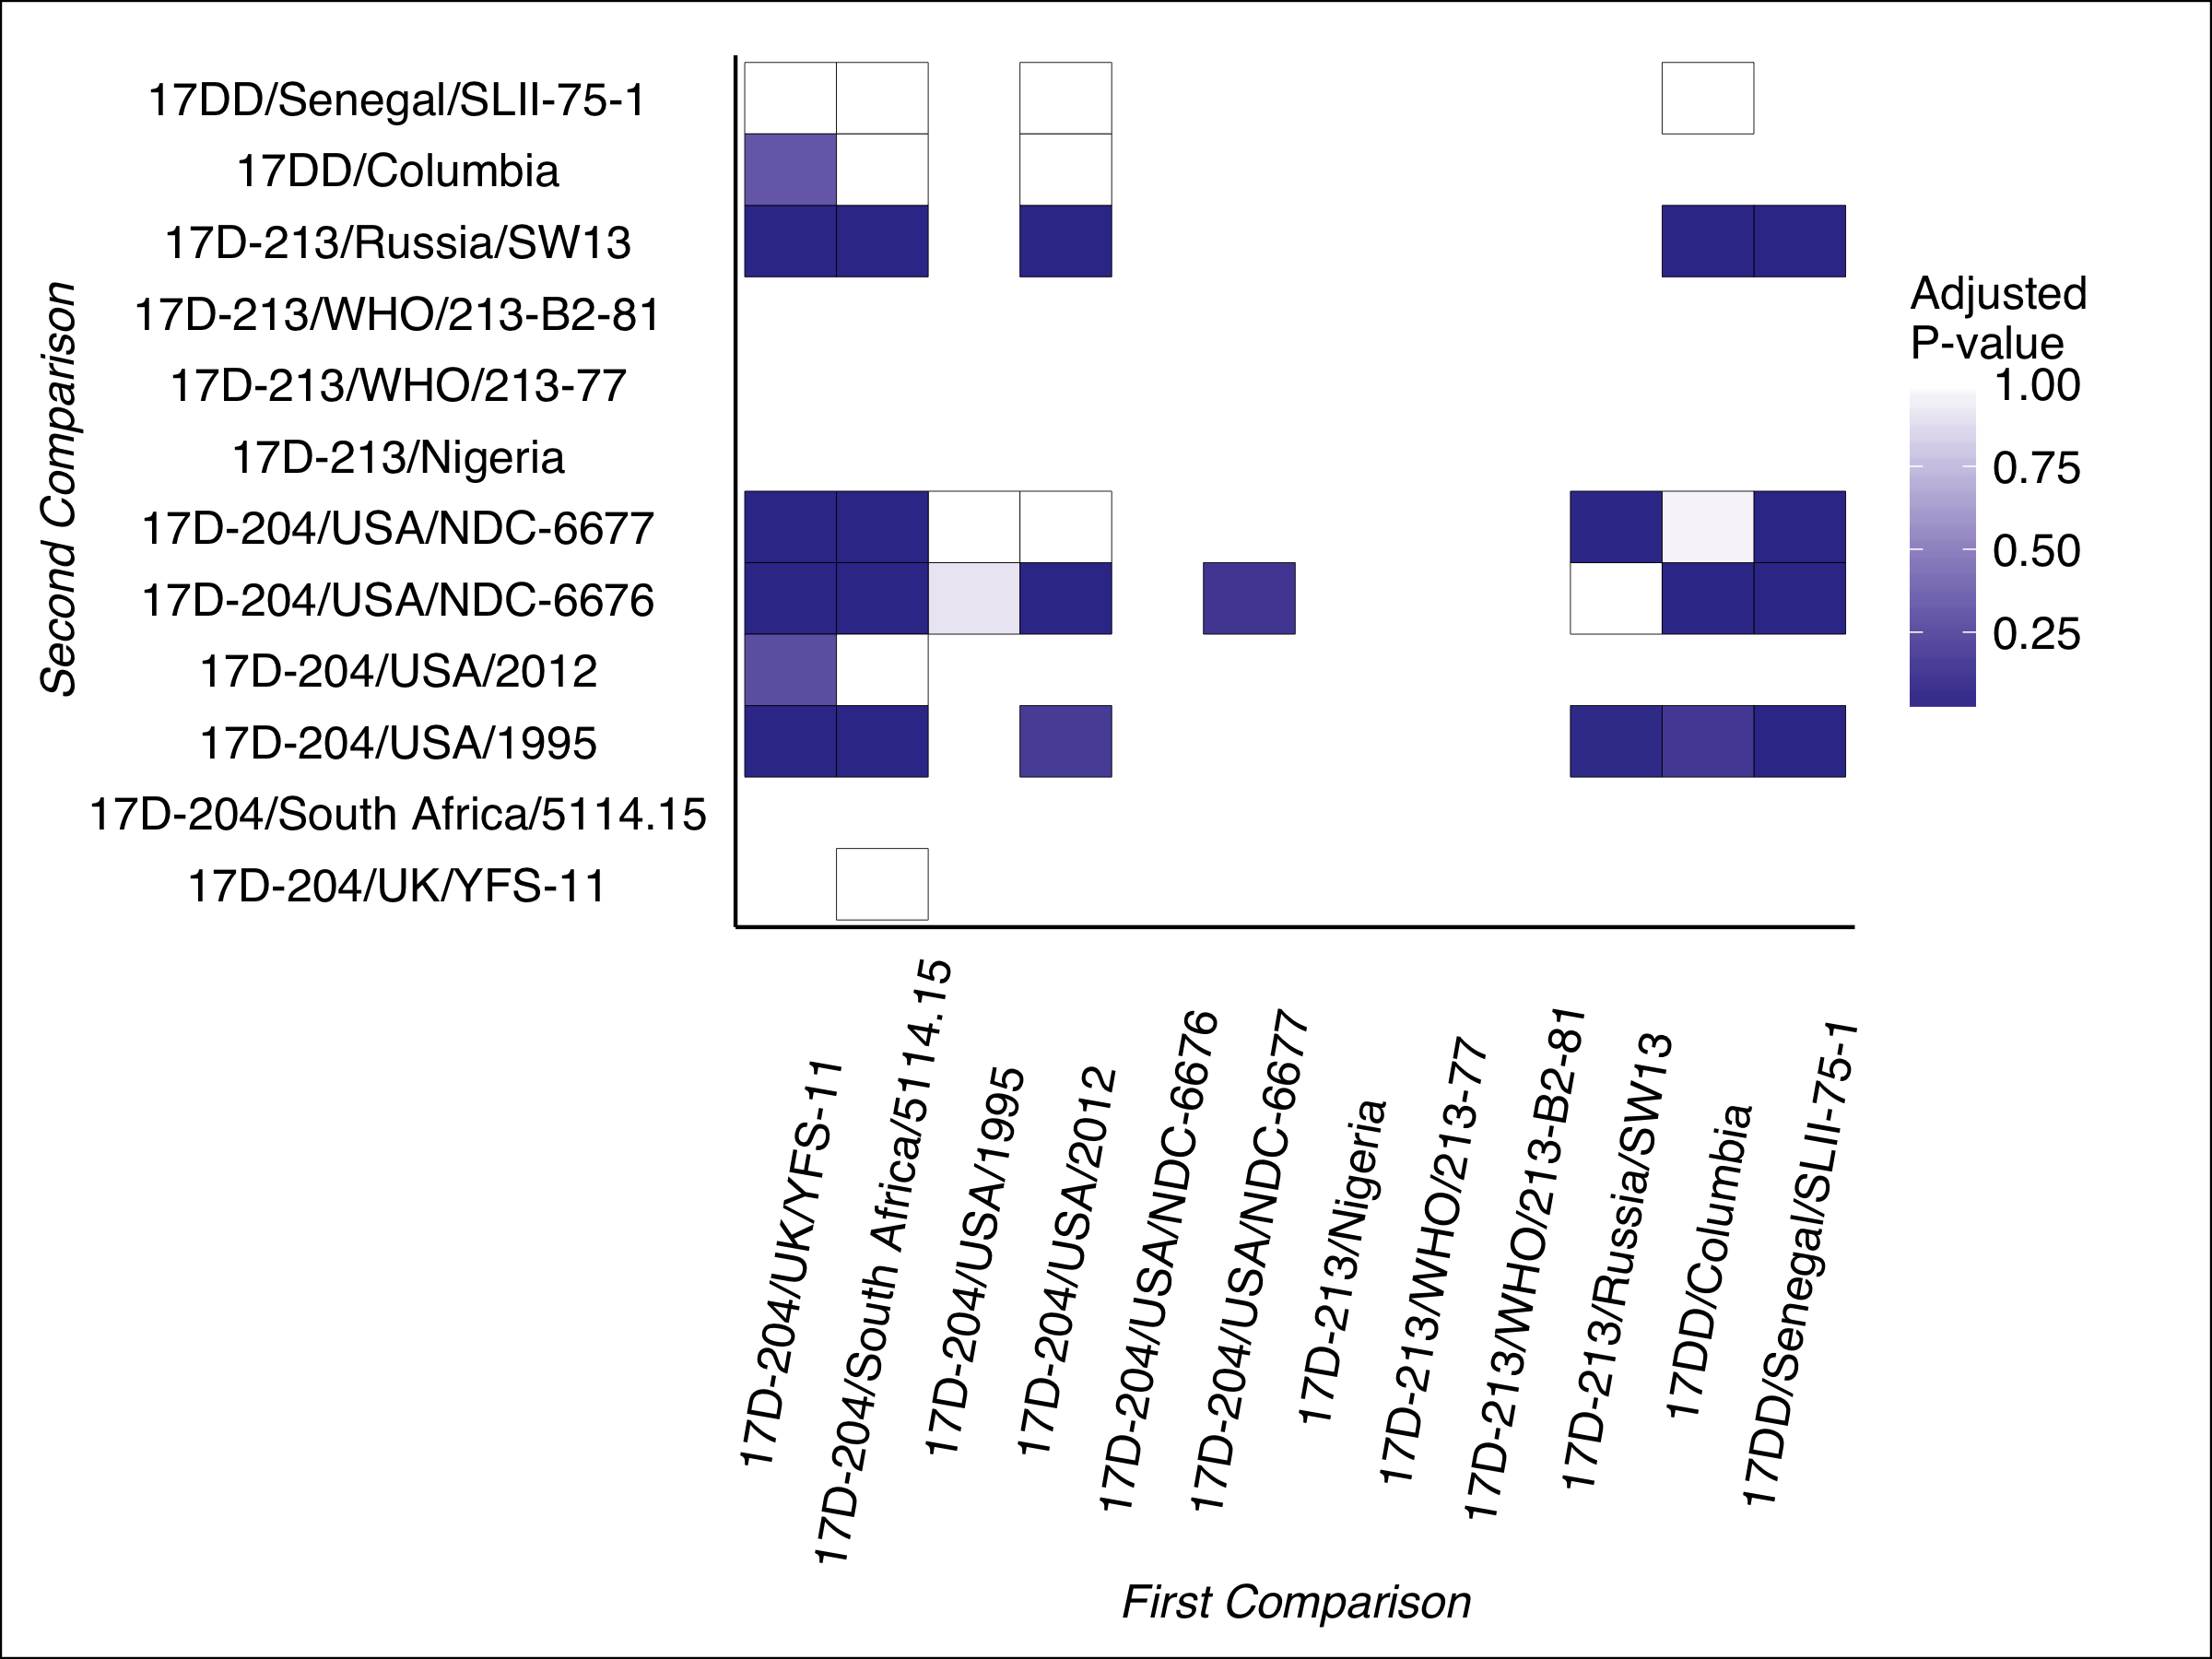
\includegraphics[width=\columnwidth]{../FIGURES/Chapter_17D_Seeds_FIGURE/kruskal_heat_FIGURE/082415_Dunns_heatmap_allsites.png}
	\caption[Heat map of Kruskal-Wallis p-values for all pairwise comparisons of normalized Shannon's entropy, considering values along the whole genome extent of each strain.]{Heat map of Kruskal-Wallis p-values for all pairwise comparisons of \gls{nse}, considering values along the whole genome extent of each strain. Dunn's post-hoc correction was used to adjust for multiple tests.}
	\label{kruskal_heat_whole}
\end{figure} 

\begin{figure}[p]
	\centering
	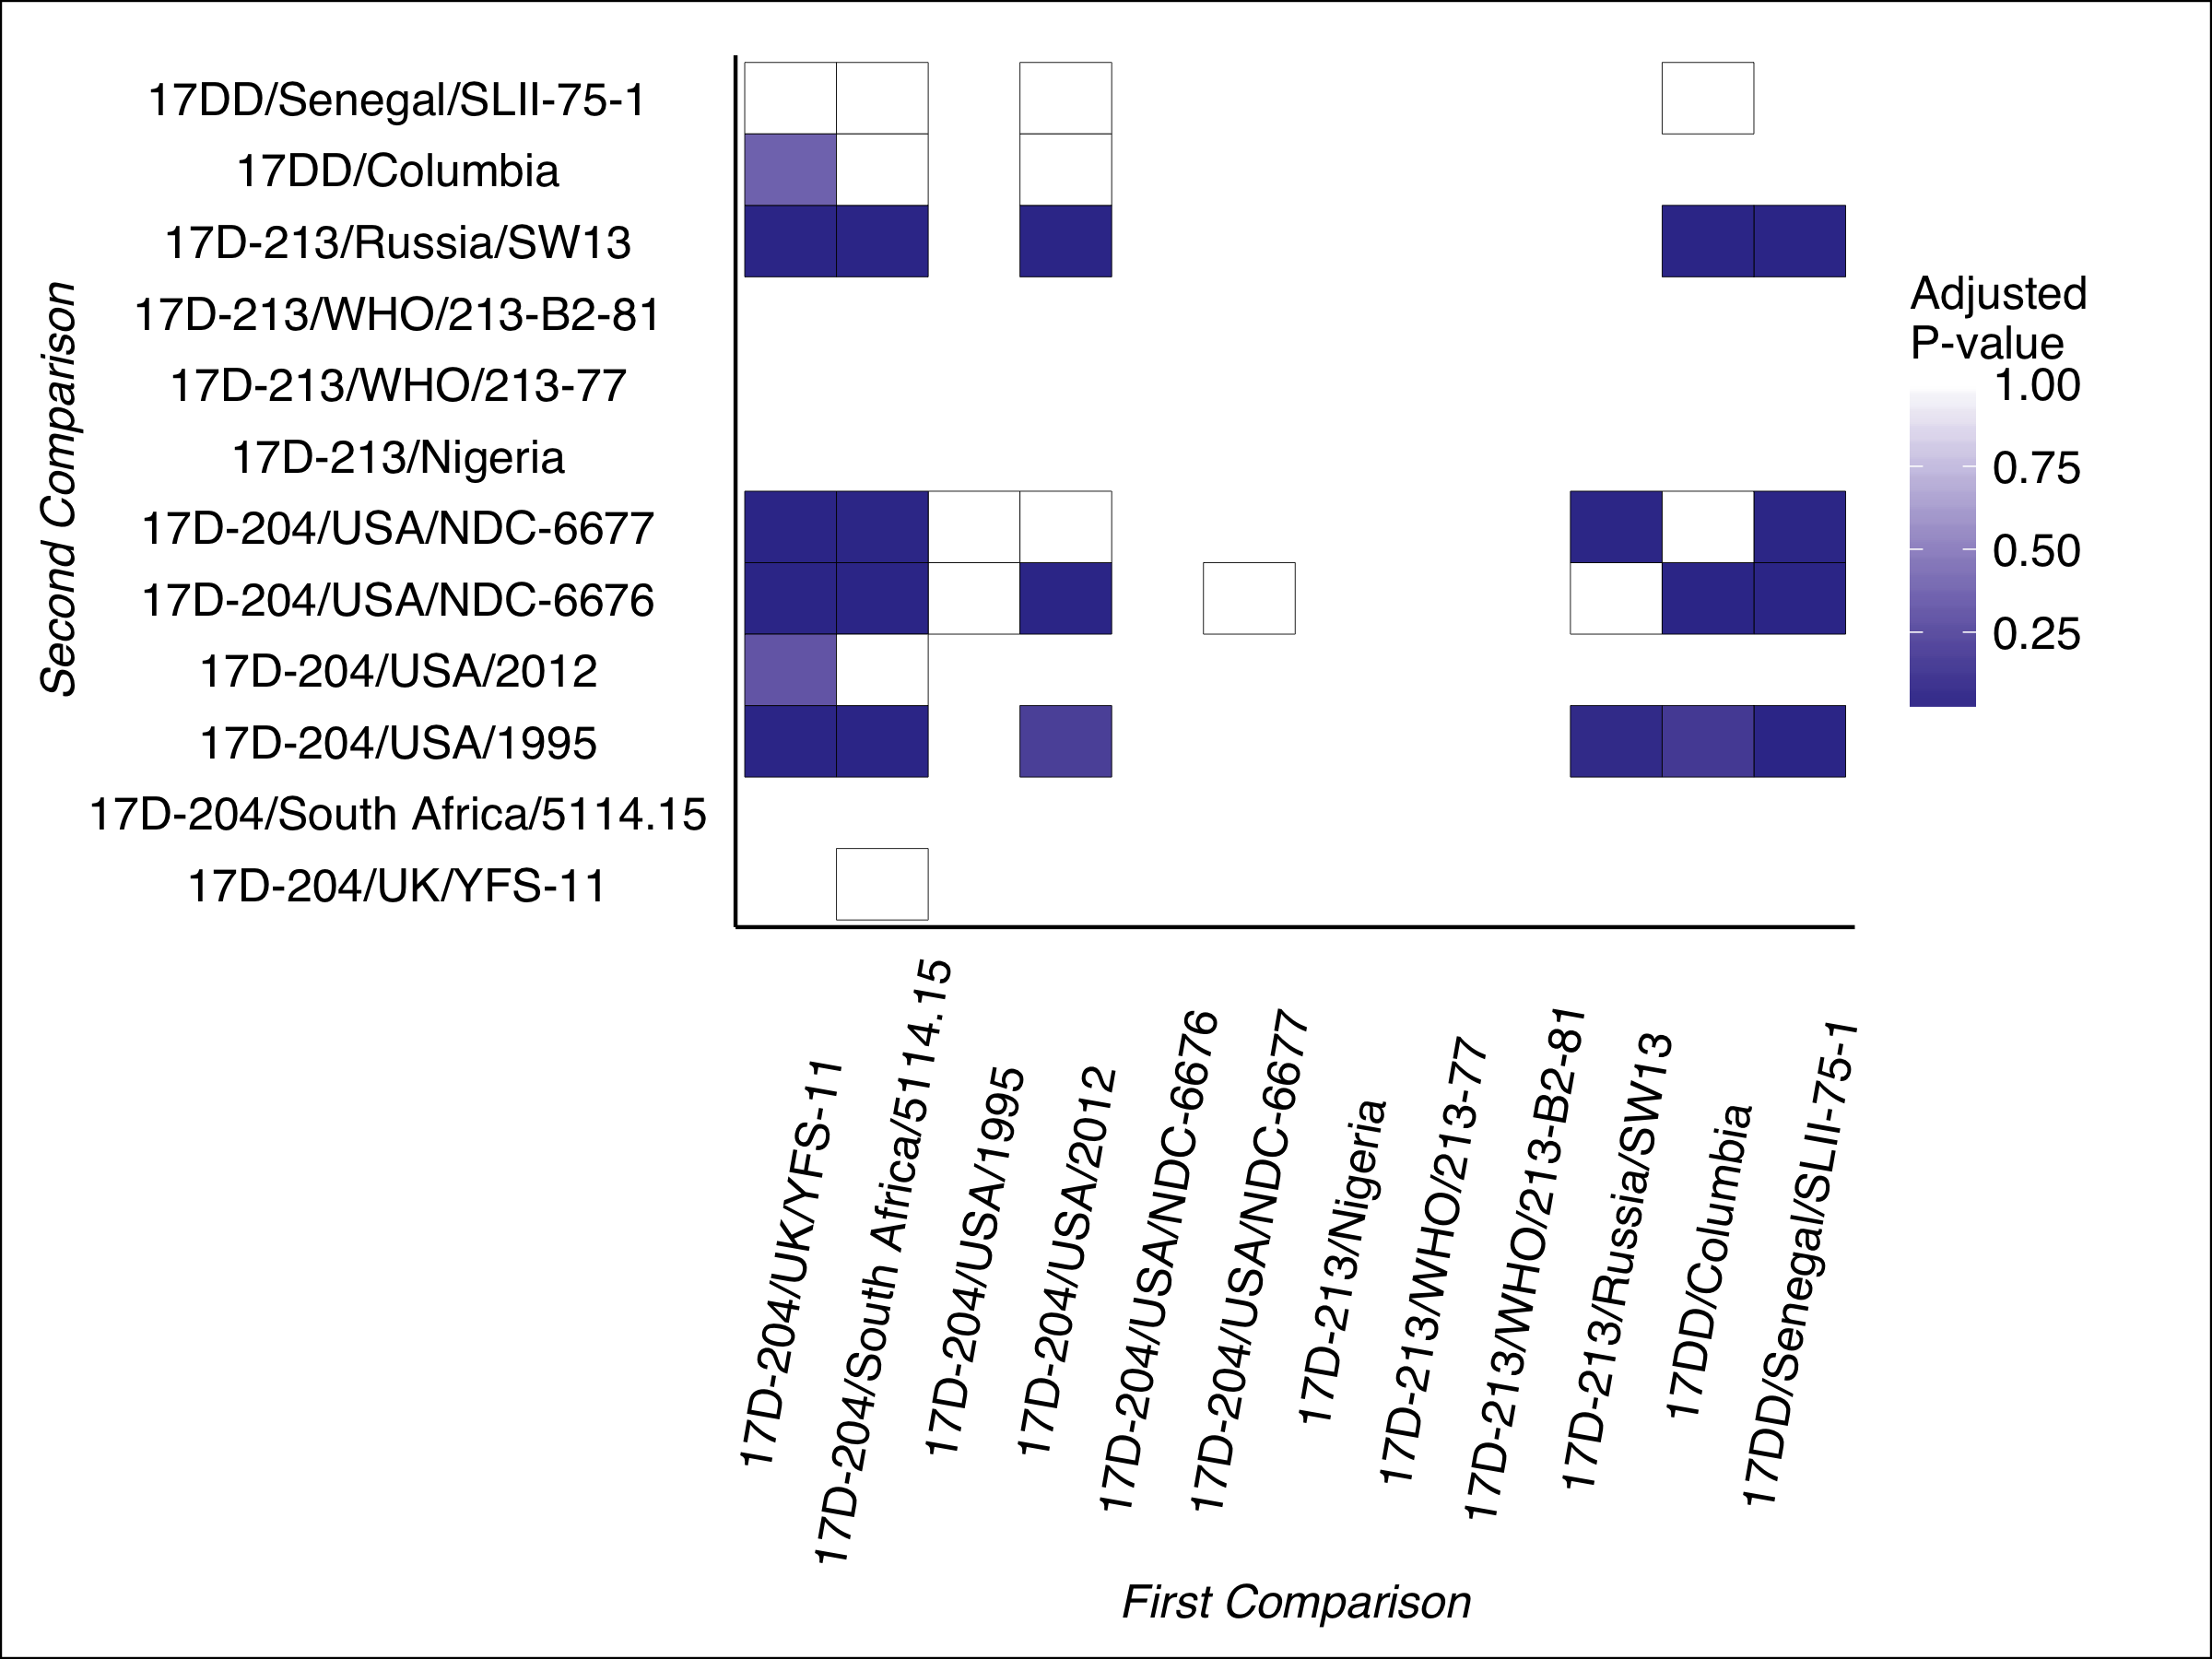
\includegraphics[width=\columnwidth]{../FIGURES/Chapter_17D_Seeds_FIGURE/kruskal_heat_ORF_FIGURE/082415_Dunns_heatmap_ORF.png}
	\caption[Heat map of Kruskal-Wallis p-values for all pairwise comparisons of normalized Shannon's entropy, considering values only along the open reading frame of each strain.]{Heat map of Kruskal-Wallis p-values for all pairwise comparisons of \gls{nse}, considering values only along the open reading frame of each strain. Dunn's post-hoc correction was used to adjust for multiple tests.}
	\label{kruskal_heat_ORF}
\end{figure} 
\clearpage

\begin{figure}[p]
	\centering
	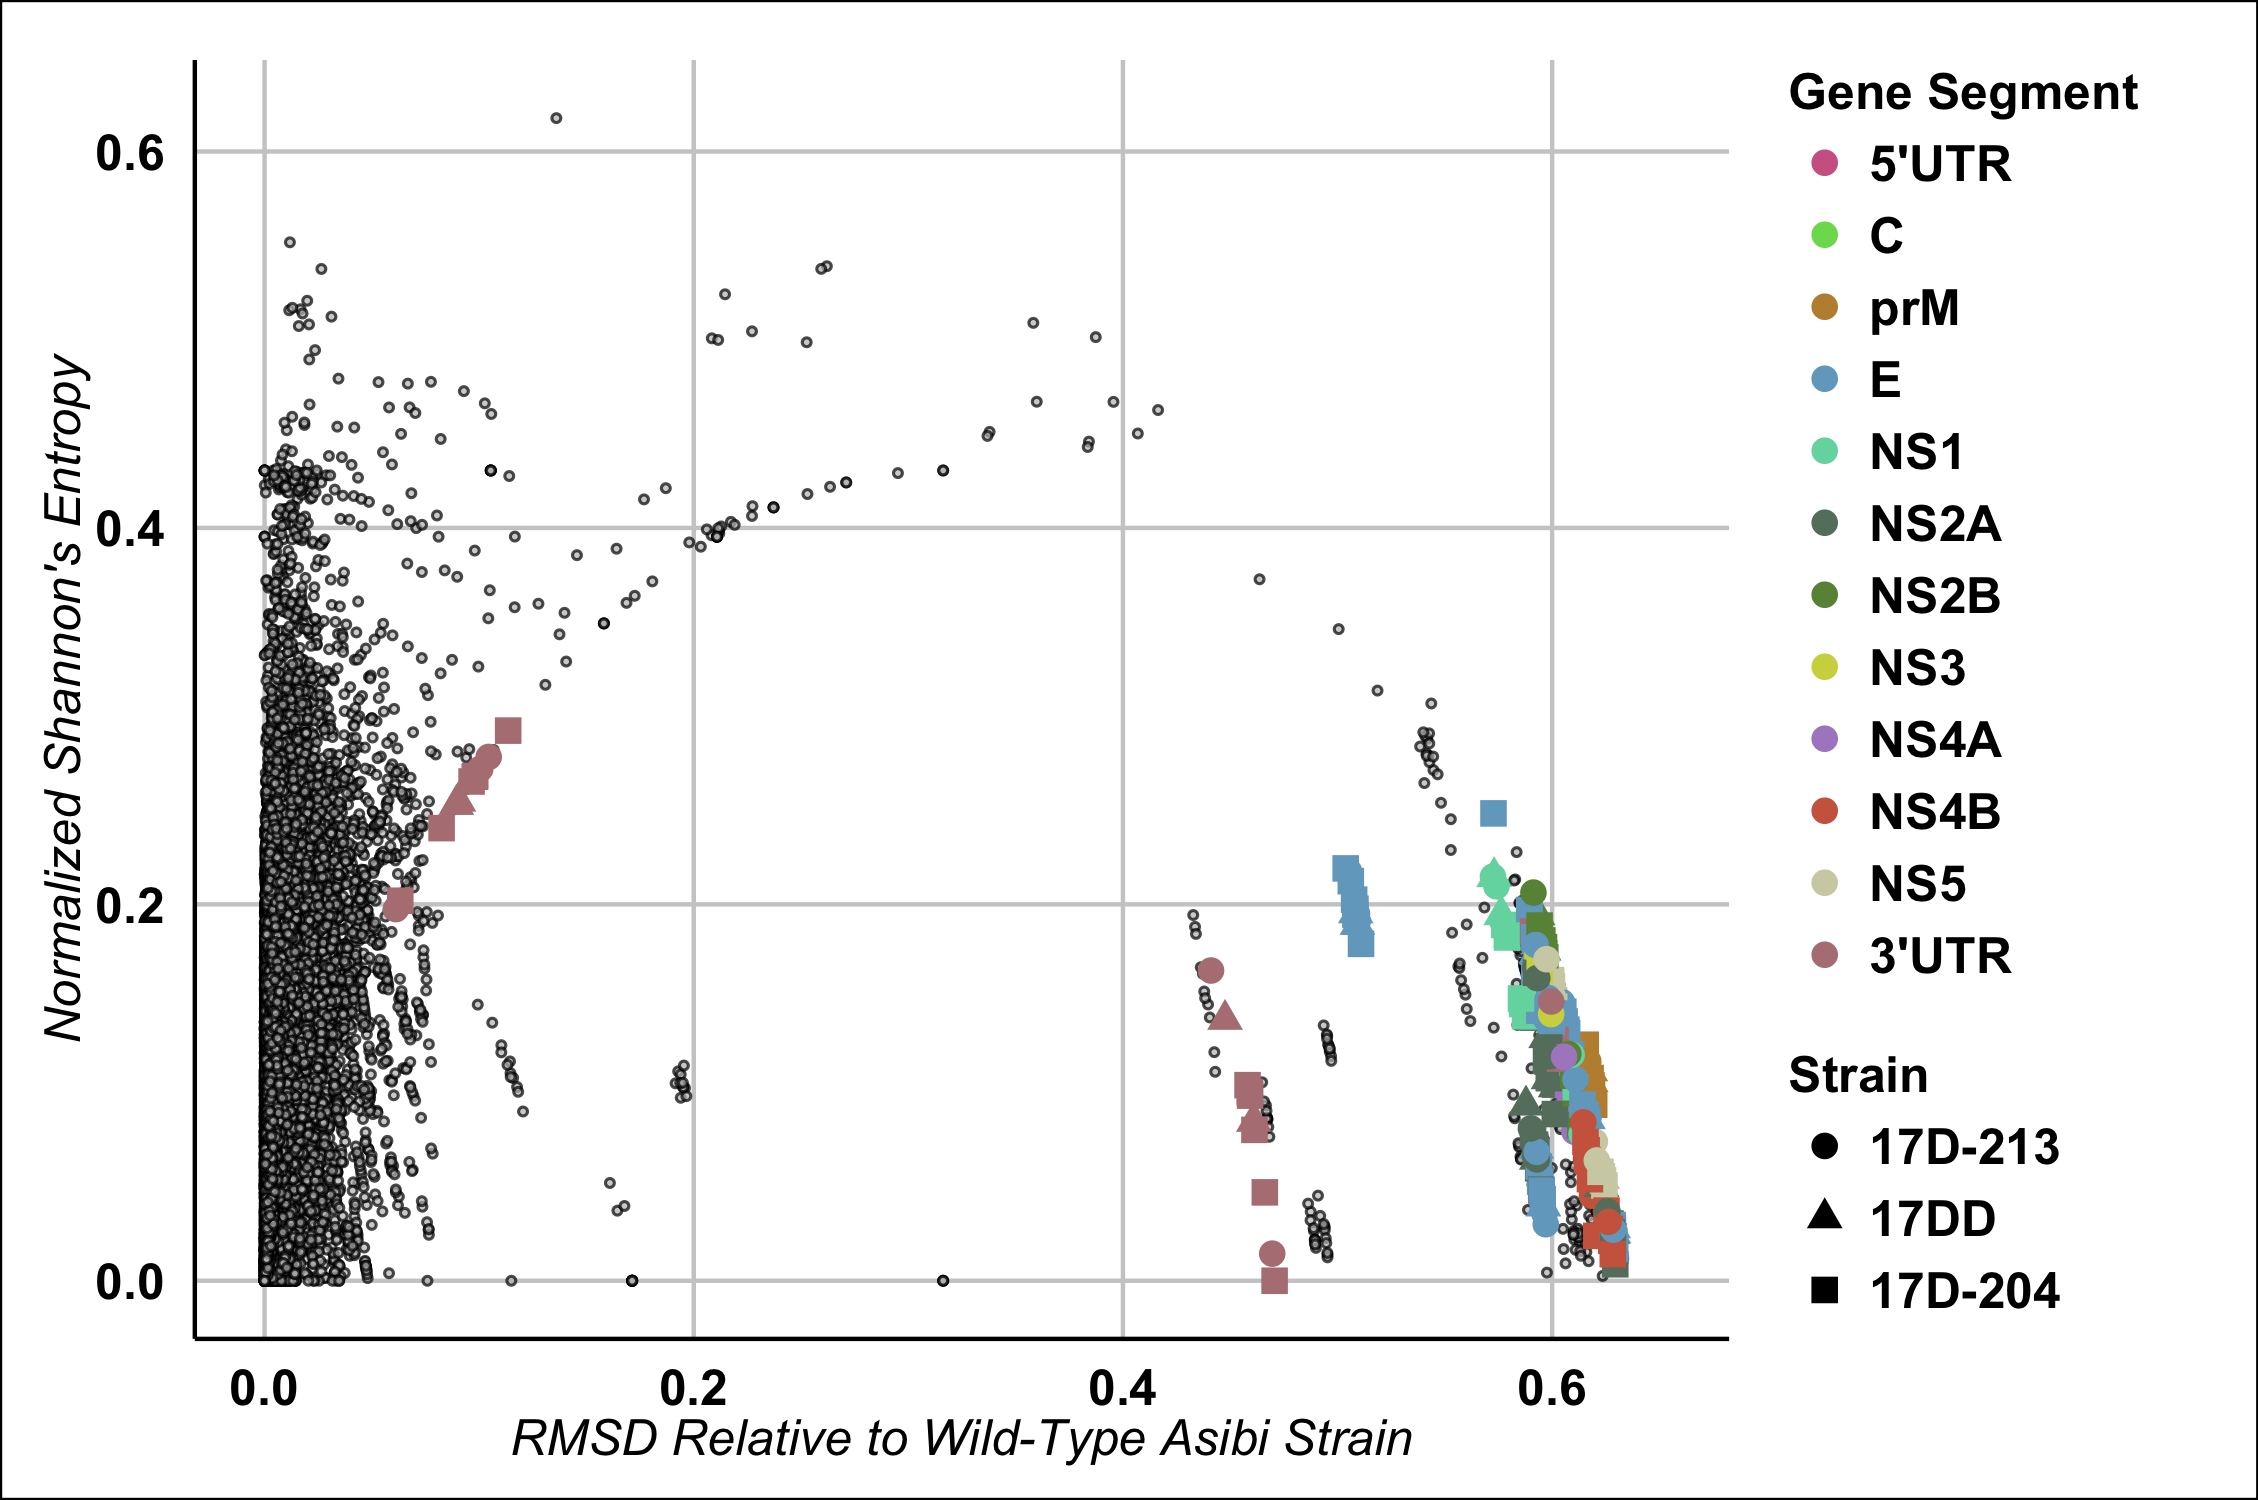
\includegraphics[width=\columnwidth]{../FIGURES/Chapter_17D_Seeds_FIGURE/scatter_distance_FIGURE/scatter_distance_STANDALONE.png}
	\caption[Scatter plot of normalized Shannon's entropy versus RMSD relative to Asibi for all nucleotide sites recovered in each strain.]{Scatter plot of \gls{nse} versus \gls{rmsd} relative to Asibi for all nucleotide sites recovered in each strain. Colored glyphs are contained in the \gls{who} standard genotype for \gls{yfv}, and specifically indicate that at the nucleotide positions described for the vaccine genotype, the nucleotide subpopulations of those sites are equivalently selected from the parental genotype for all vaccine strains.}
	\label{scatter_distance_seeds}
\end{figure} 
\clearpage

\begin{figure}[p]
	\centering
	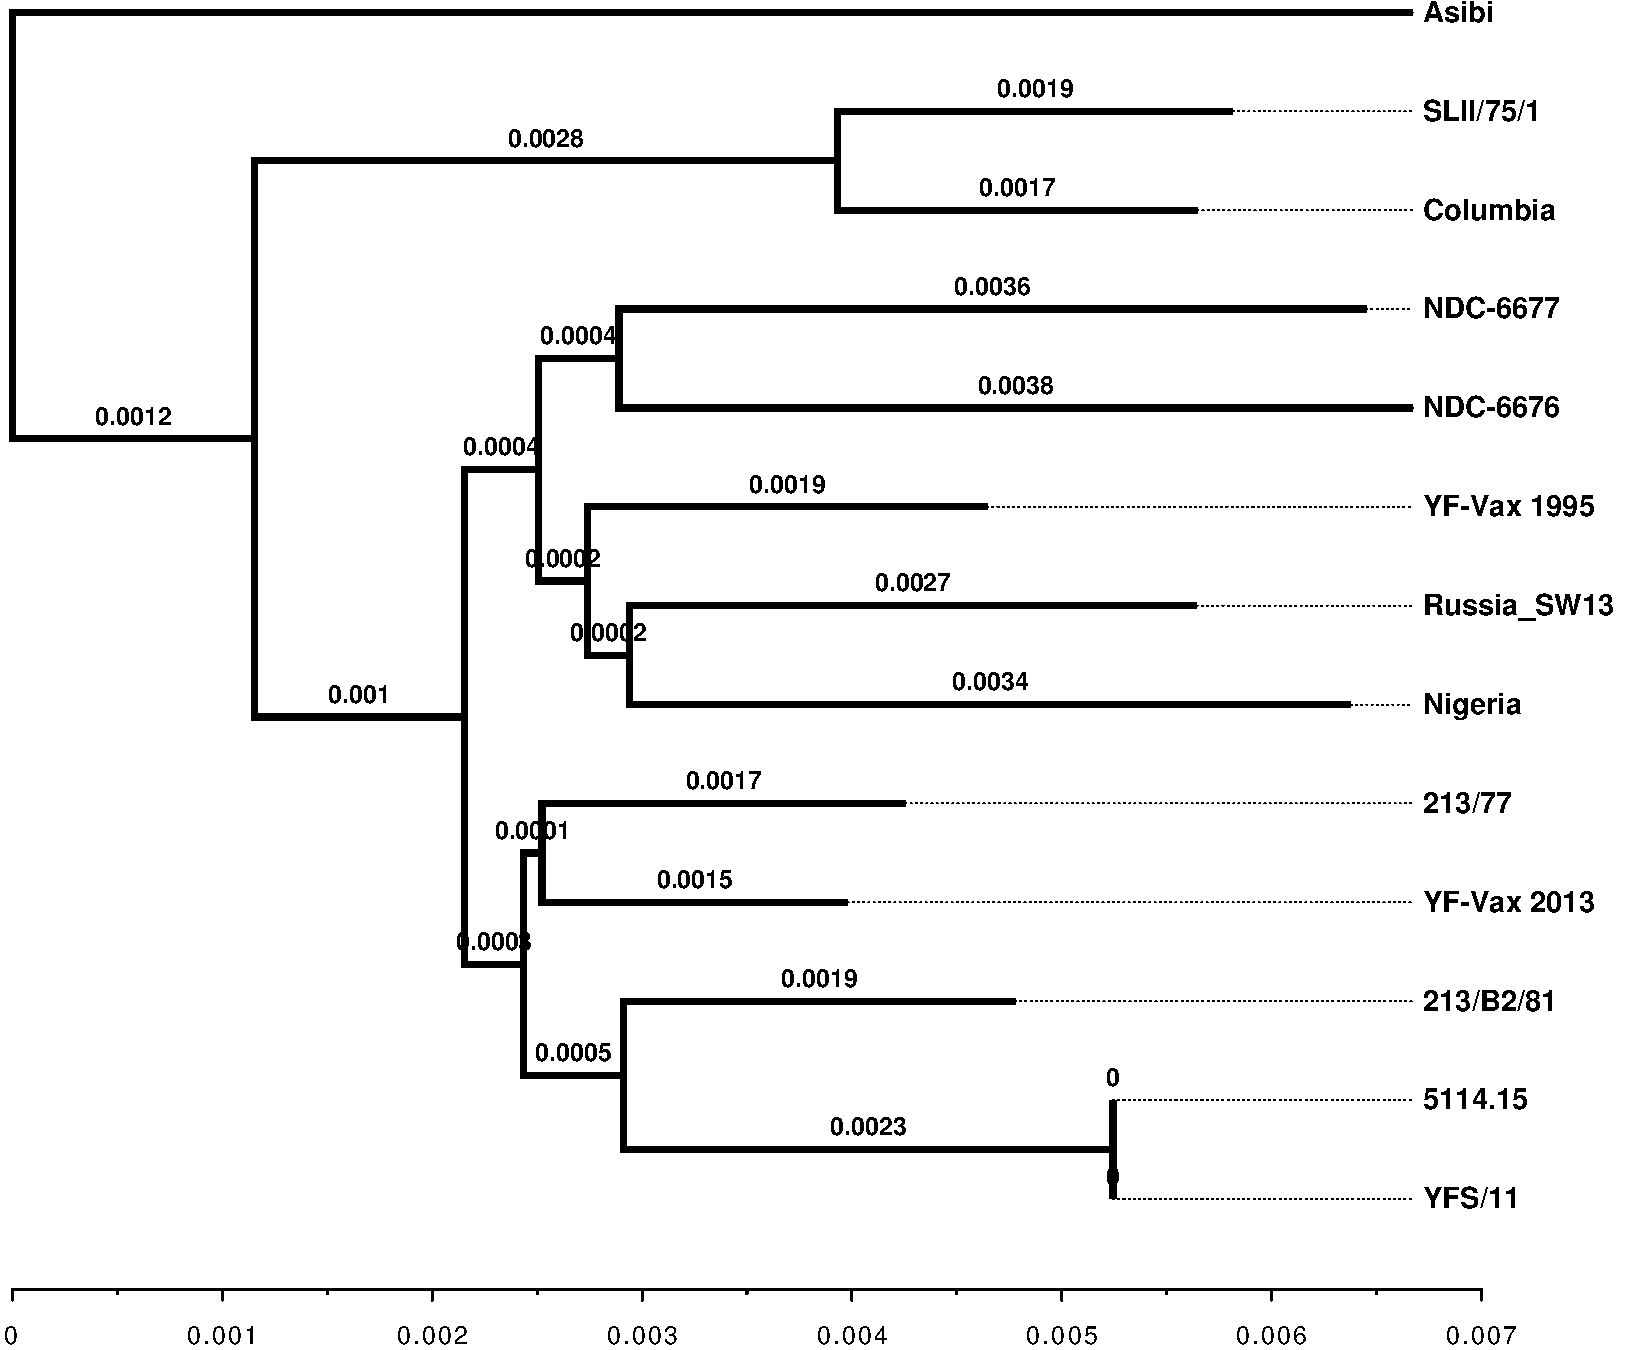
\includegraphics[width=\columnwidth]{../FIGURES/Chapter_17D_Seeds_FIGURE/ngs_phylogeny_FIGURE/ngs_phylogeny_STANDALONE.pdf}
	\caption[Neighbor-joining phylogeny calculated by pairwise mean RMSD for all seeds considered in the study.]{Neighbor-joining phylogeny calculated by pairwise mean \gls{rmsd} for all seeds considered in the study. A pairwise matrix of \gls{rmsd} was constructed and used as the distance measurement from which the branch lengths were derived.}
	\label{NGS_phylo_seeds}
\end{figure} 
\clearpage

\begin{figure}[p]
	\centering
	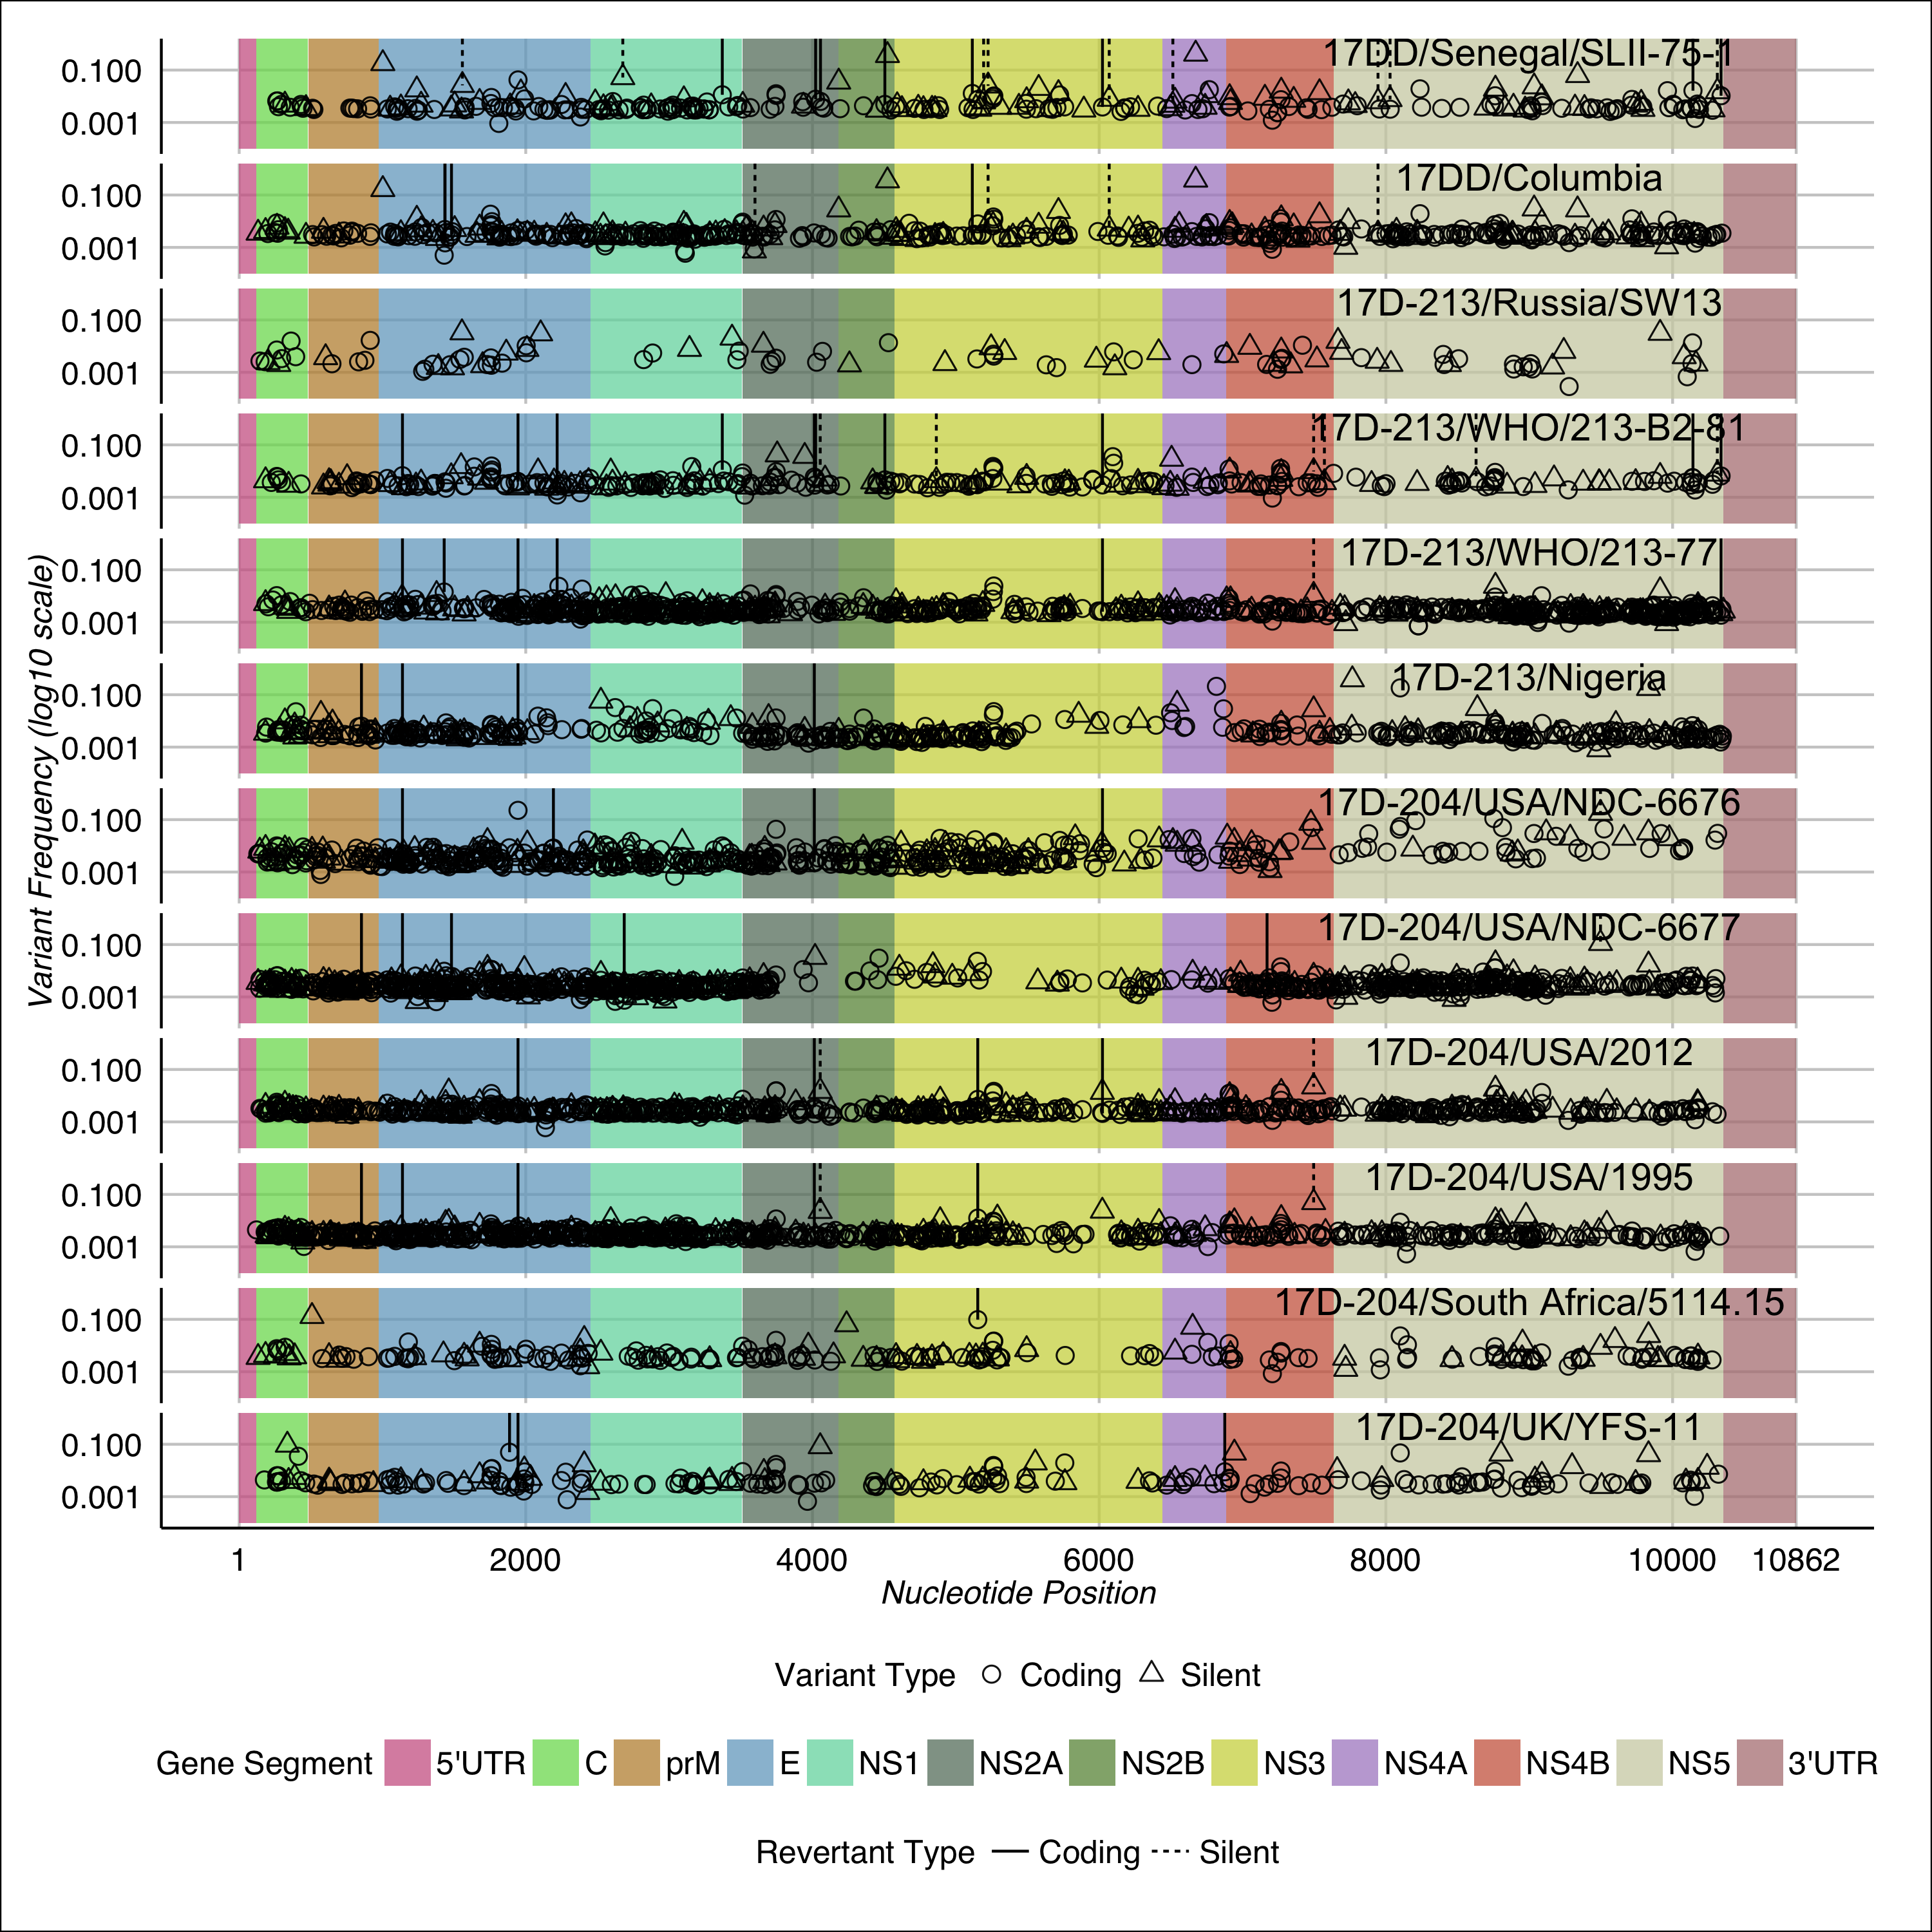
\includegraphics[width=\columnwidth]{../FIGURES/Chapter_17D_Seeds_FIGURE/vphaser_complete_FIGURE/vphaser_complete_STANDALONE.png}
	\caption[Modeled variants for the strains, with coding/silent classifications and wild-type revertants indicated.]{Modeled variants for the strains, with coding/silent classifications and wild-type revertants indicated. \Glspl{snv} are plotted as frequency against nucleotide position in the read alignment. Coding and silent variants were classified against the consensus sequences of each respective strain, and are differentiated by glyph shape. Vertical lines indicate \glspl{snv} that represent subpopulation revertants to the wild-type genotype, and are likewise classified as coding or silent.}
	\label{vphaser_seeds}
\end{figure} 
\clearpage

\begin{figure}[p]
	\centering
	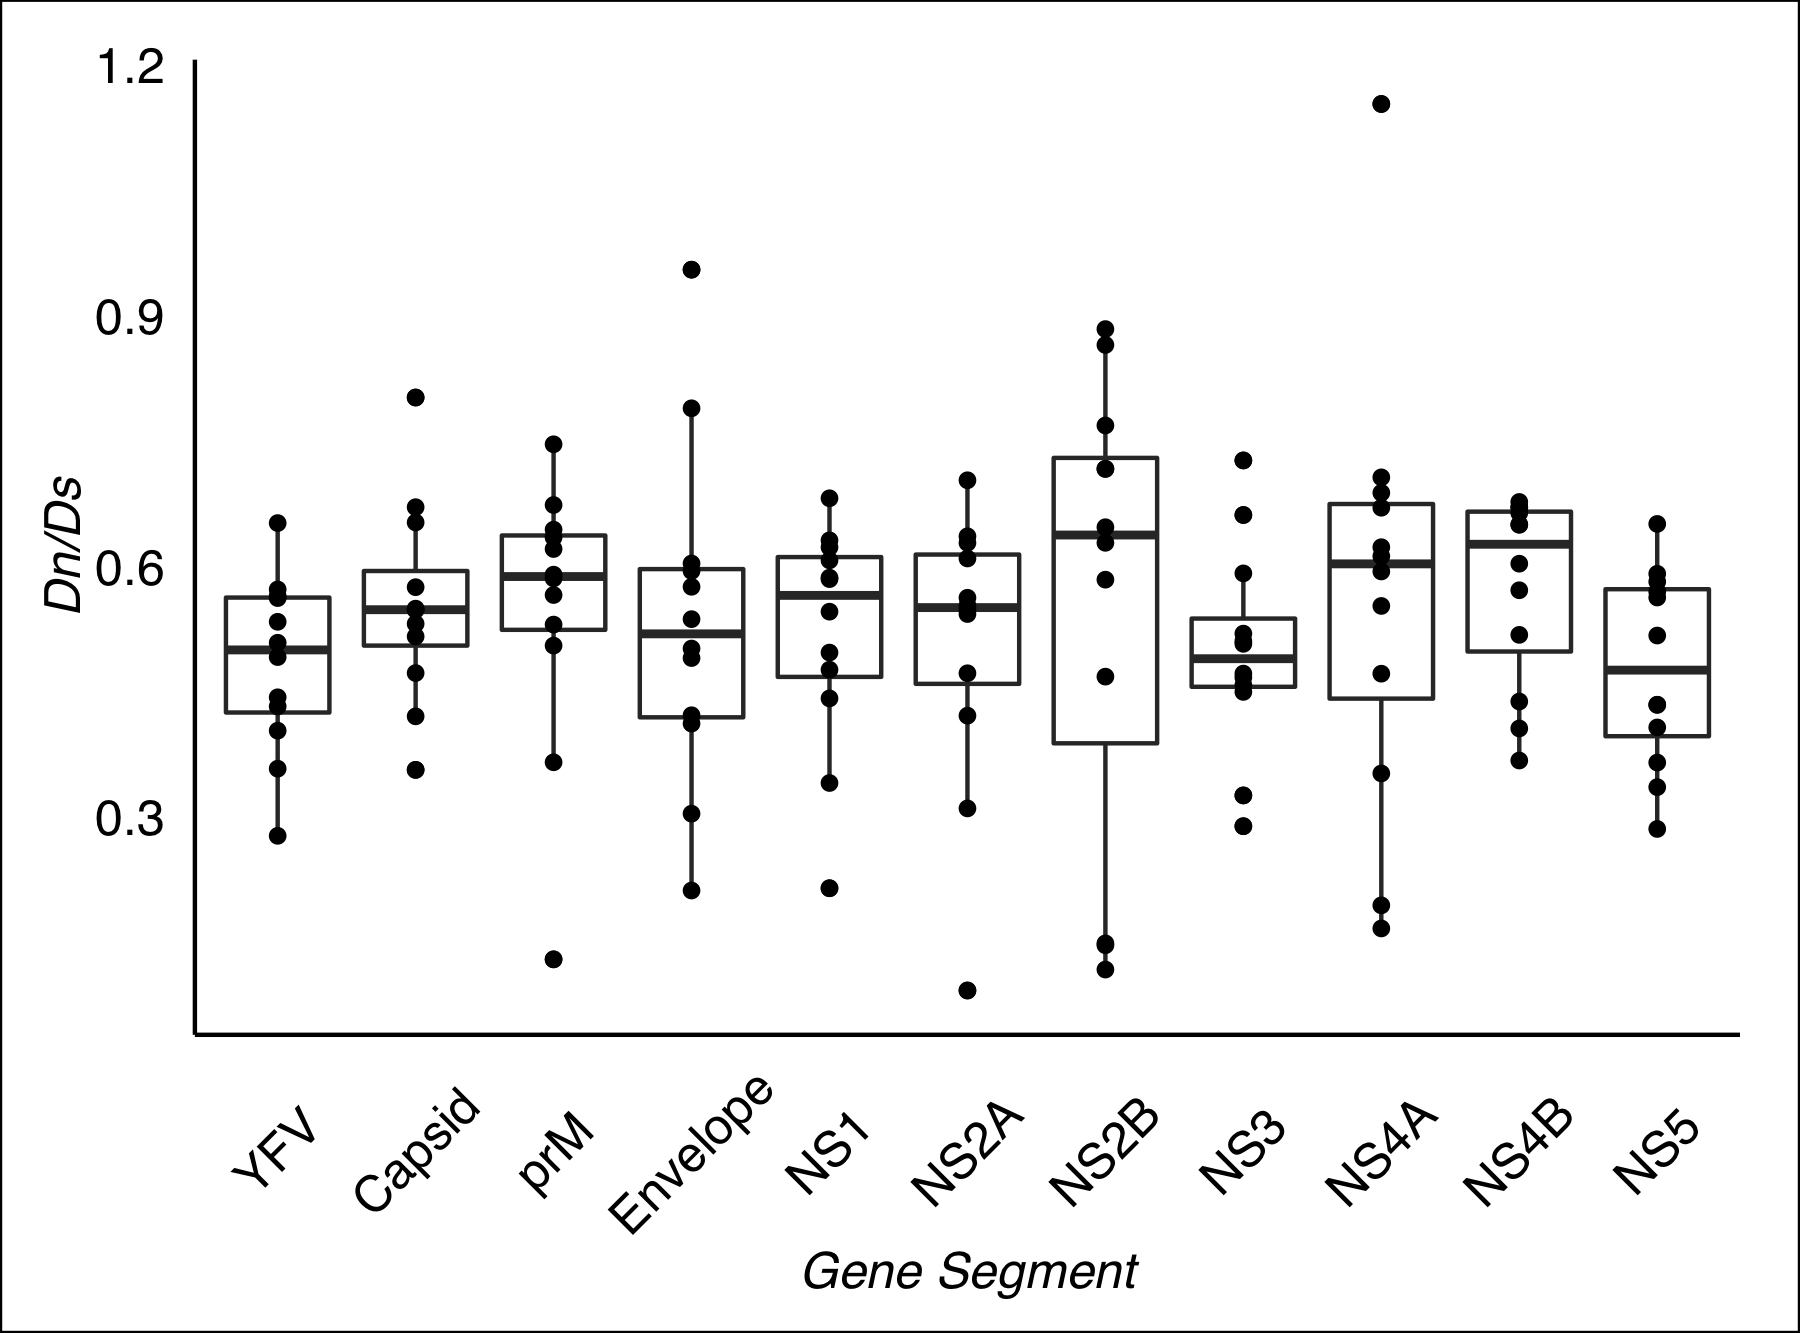
\includegraphics[width=\columnwidth]{../FIGURES/Chapter_17D_Seeds_FIGURE/dnds_boxplot_FIGURE/dnds_boxplot_STANDALONE.png}
	\caption[Boxplots of summarized $dN/dS$ values along each gene segment.]{Boxplots of summarized $dN/dS$ values along each gene segment. All box plots depict the median, first quartile, third quartile, with whiskers showing +/- 1.5 times the interquartile distance.}
	\label{dnds_boxlot_seeds}
\end{figure} 
\clearpage

\begin{figure}[p]
	\centering
	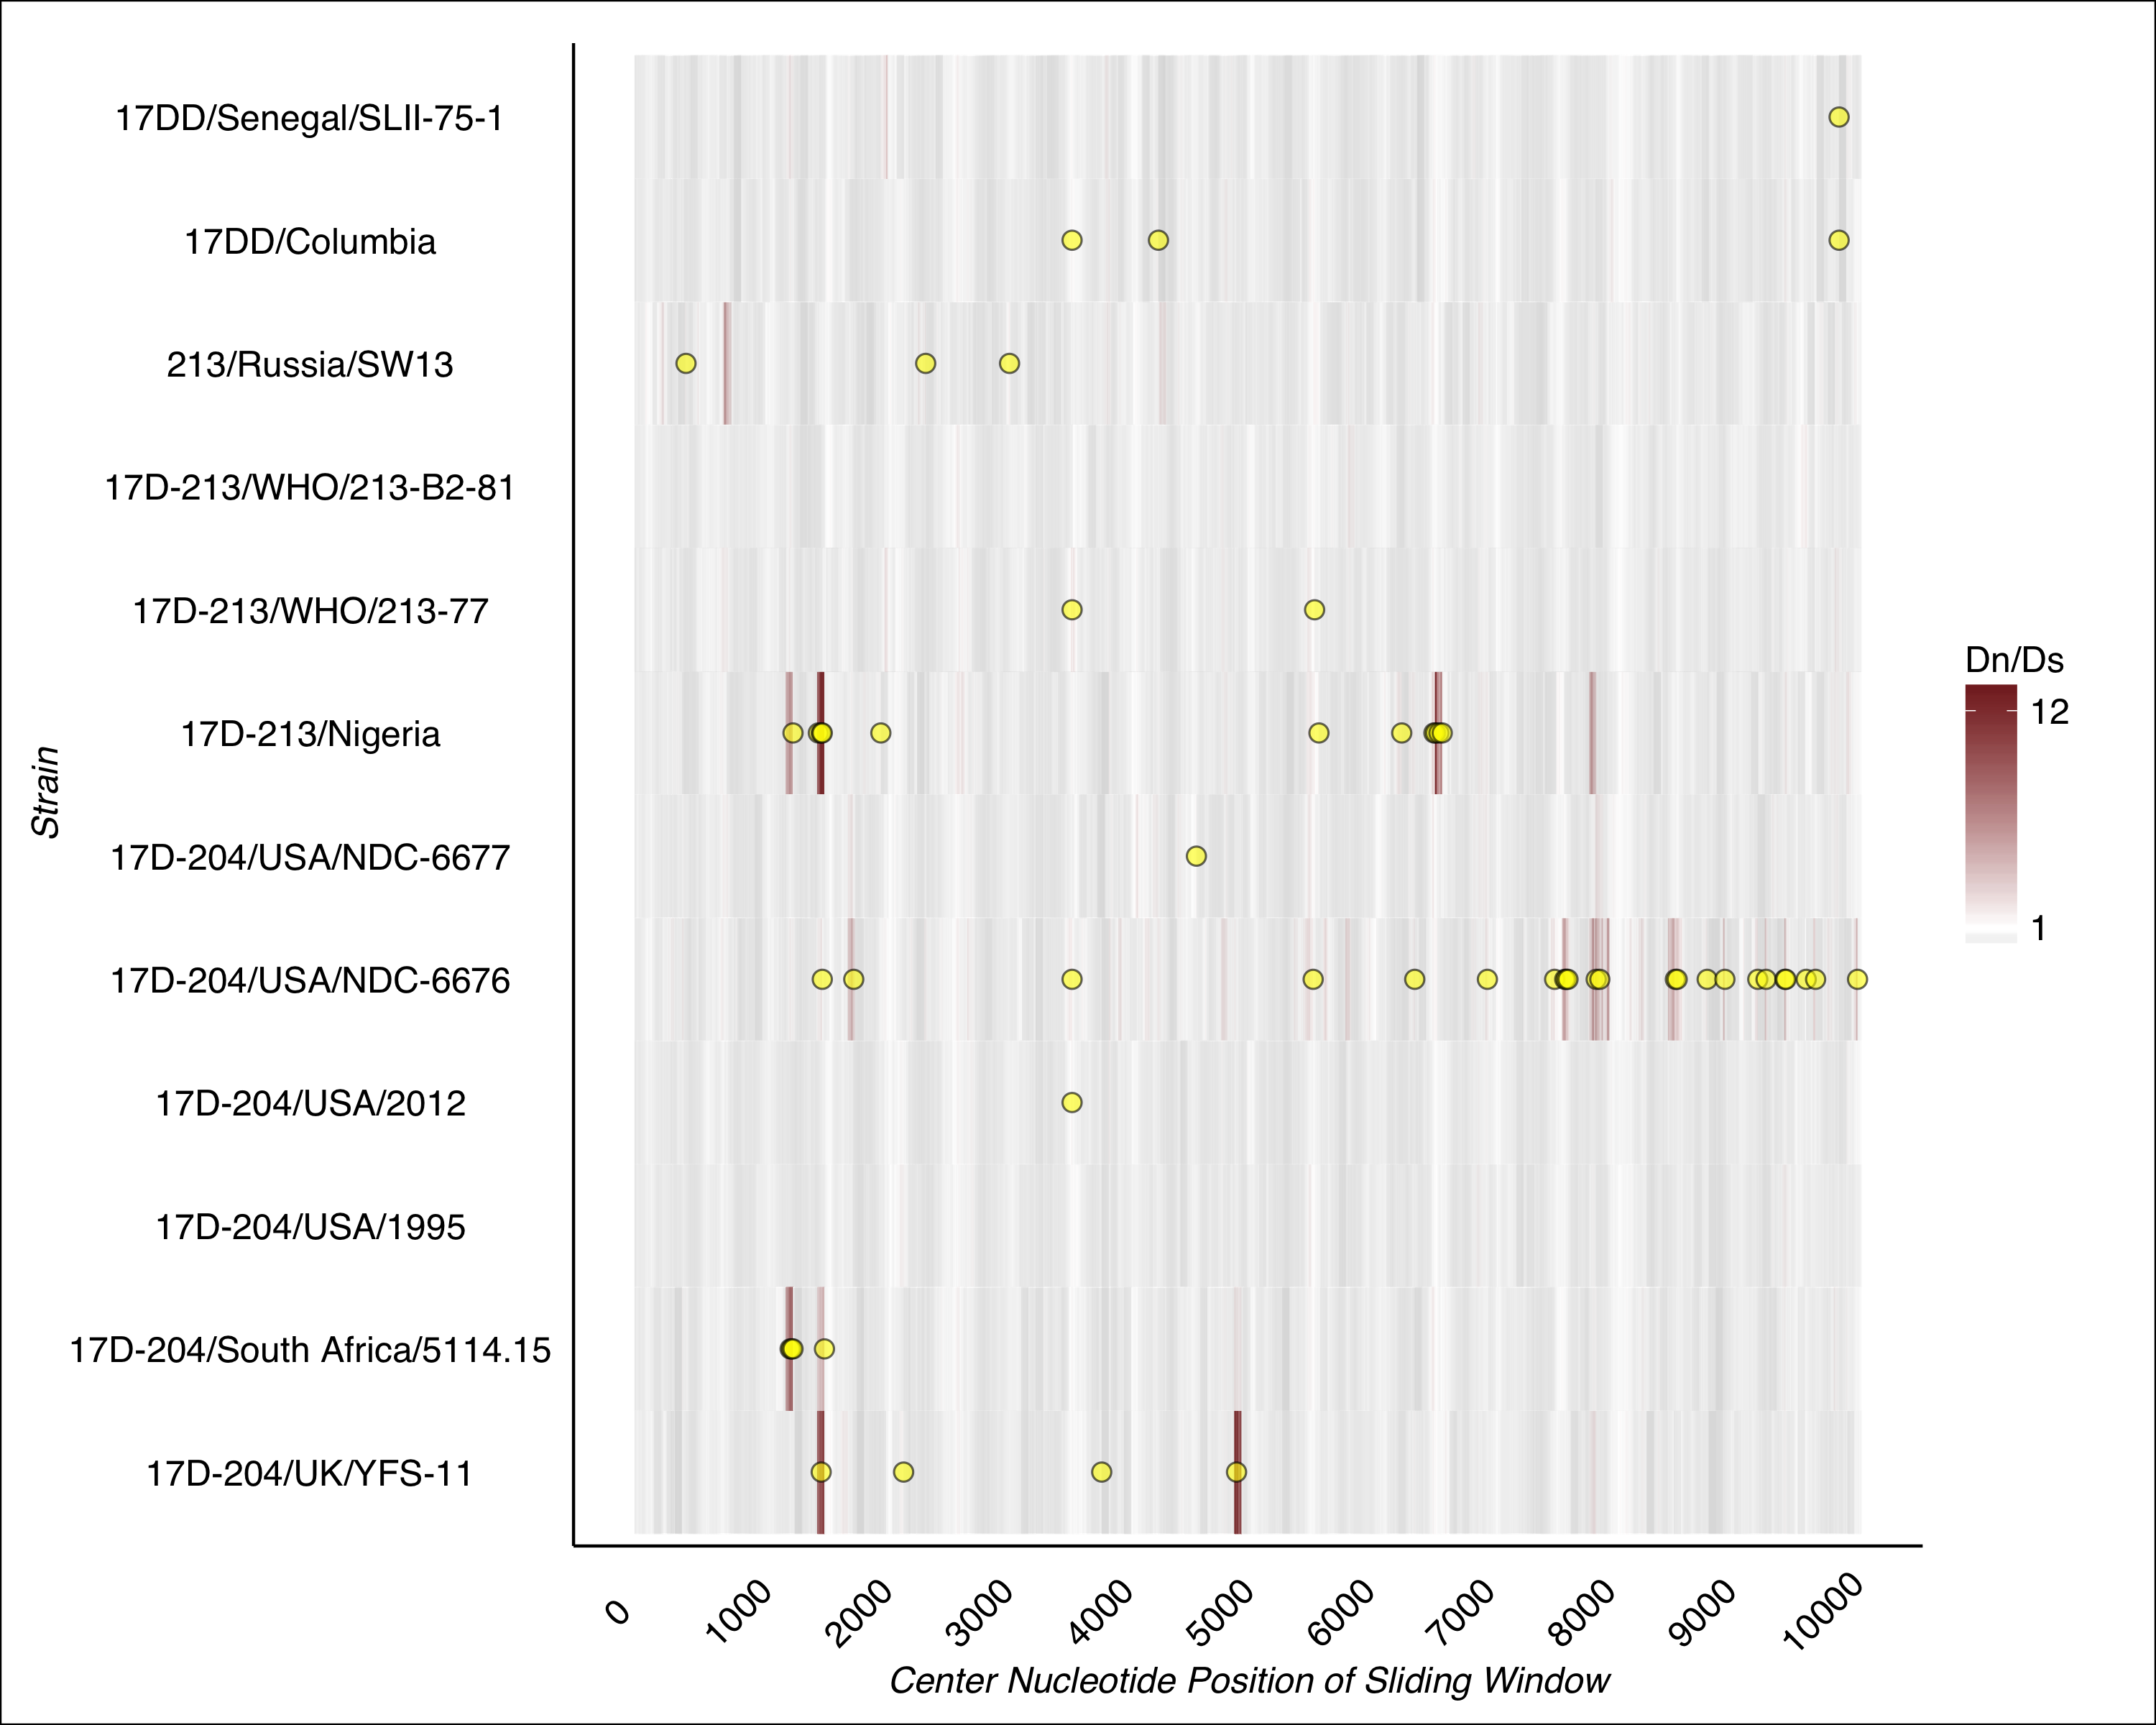
\includegraphics[width=\columnwidth]{../FIGURES/Chapter_17D_Seeds_FIGURE/dnds_heat_FIGURE/dnds_heat_STANDALONE.png}
	\caption[Heatplot of $dN/dS$ values for all strains considered.]{Heatplot of $dN/dS$ values for all strains considered. Color scale indicates increasing $dN/dS$ for 20-codon windows, generated with a sliding window step size of single-codon distance.}
	\label{dnds_heat_seeds}
\end{figure} 
\clearpage

\begin{figure}[p]
	\centering
	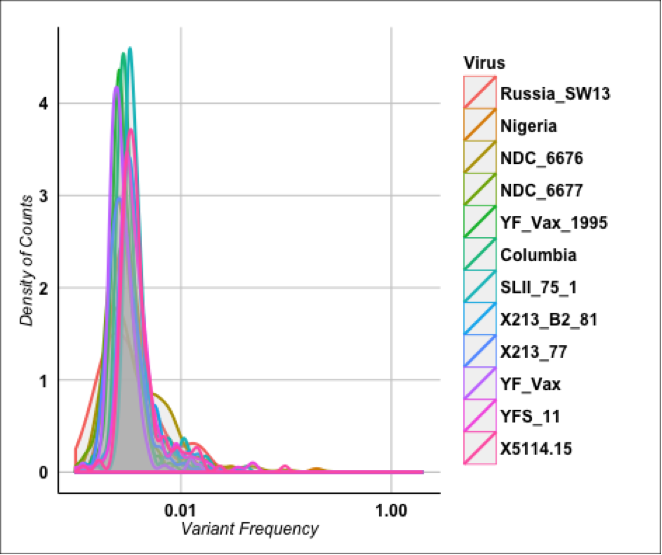
\includegraphics{../FIGURES/Chapter_17D_Seeds_FIGURE/density_plot_FIGURE/density_plot_STANDALONE.png}
	\caption[Density plot for counts of variants, derived from modeled SNVs in the population.]{Density plot for counts of variants, derived from modeled \glspl{snv} in the population. The curves show a typical pattern for low-diversity viral populations, which is that of a large population of small-frequency variants (the high density area at left in the plot), with a low population count of higher-frequency variants in the tail of the distribution. Curves overlap considerably, visualizing that all of the vaccine strains analyzed exhibit this type of similarity.}
	\label{density_plot_seeds}
\end{figure}
\clearpage

